\documentclass[11pt]{article}
\usepackage[margin=1in]{geometry} % Adjust margins as needed
%!TEX root = ./main_source.texx
\UseRawInputEncoding
\usepackage{hyperref}
% For authors with multiple institutions
\usepackage[affil-sl]{authblk}
% For line-numbers in my document
\usepackage{lineno}

% Redefine the cite color to your preferred color

\usepackage[utf8]{inputenc}
\usepackage[T1]{fontenc}
\usepackage{anyfontsize}
\usepackage{lipsum} % For dummy text
\usepackage{microtype} % Improved font rendering
\usepackage{titlesec} % Customize section titles
\usepackage{graphicx} % For including images
\usepackage{bm}
\usepackage{svg}
\usepackage{xcolor}
% \usepackage{ulem}
\usepackage{bbm}
\usepackage{xspace}
\usepackage{tabularx}
\usepackage{stmaryrd}
\SetSymbolFont{stmry}{bold}{U}{stmry}{m}{n}
\usepackage{bbm}
\usepackage{url}            % simple URL typesetting
\usepackage{booktabs}       % professional-quality tables
\usepackage{amsfonts}       % blackboard math symbols
\usepackage{nicefrac}       % compact symbols for 1/2, etc.
\usepackage{microtype}      % microtypography
\usepackage{amsmath,amsthm}
\usepackage{tikz}
\usepackage[most]{tcolorbox}

\usepackage{natbib}
% \bibliographystyle{dinat}
% \setcitestyle{authoryear, open={[},close={]}} %Citation-related commands

%\usepackage{amssymb}
\let\Bbbk\relax
\usepackage{newtxmath}
\usepackage{letltxmacro}
\usepackage{bm}

\usepackage{soul}
\usepackage[linesnumbered,ruled,vlined]{algorithm2e}
\usepackage[compatible]{algpseudocode} 
\usepackage{bbm}
\usepackage{svg}
\usepackage{xcolor}
\usepackage{xspace}
\usepackage{stmaryrd}
\usepackage{bbm}
\usepackage{url}            % simple URL typesetting
\usepackage{booktabs}       % professional-quality tables
\usepackage{nicefrac}       % compact symbols for 1/2, etc.
\usepackage{microtype}      % microtypography
\usepackage{letltxmacro}
\usepackage{bm}
\usepackage{caption}
\usepackage{subcaption}
\usepackage{soul}
\usepackage[linesnumbered,ruled,vlined]{algorithm2e}
\usepackage[compatible]{algpseudocode} 
% \usepackage{pgfplots}
\usepackage{doi}
\usepackage{fancyvrb,cprotect}
\usepackage{centernot}
\usepackage{fancyhdr}
\graphicspath{ {assets/} }


\definecolor{amber}{rgb}{1.0, 0.49, 0.0}
\definecolor{cadmiumgreen}{rgb}{0.0, 0.42, 0.24}
\definecolor{darkcyan}{rgb}{0.0, 0.55, 0.55}
\definecolor{darkcoral}{rgb}{0.8, 0.36, 0.27}
\definecolor{azure}{rgb}{0.0, 0.5, 1.0}
\definecolor{bittersweet}{rgb}{1.0, 0.44, 0.37}
\definecolor{razzmatazz}{rgb}{0.89, 0.15, 0.42}
\definecolor{ballblue}{rgb}{0.13, 0.67, 0.8}
\definecolor{purple}{rgb}{0.2, 0.2, 0.6}
\definecolor{egyptianblue}{rgb}{0.06, 0.2, 0.65}
\definecolor{darkslategray}{rgb}{0.0, 0.29, 0.29}
\definecolor{bananayellow}{rgb}{1.0, 0.88, 0.21}
\definecolor{blue-violet}{rgb}{0.54, 0.17, 0.89}
\definecolor{carminepink}{HTML}{EF58A0}
\definecolor{titlecolor}{RGB}{0,74,147}
\definecolor{sectioncolor}{RGB}{0,129,255}
\definecolor{subsectioncolor}{RGB}{0,129,255}
\definecolor{definitioncolor}{rgb}{0.89, 0.0, 0.13}
\usepackage{hyperref} 

\hypersetup{
    colorlinks=true,
    linkcolor=cadmiumgreen,
    citecolor=carminepink, % Set color for citation links
    urlcolor=titlecolor % Set color for URL links
}

\newcommand{\highlight}[1]{\color{razzmatazz} #1 \color{black}}
\newcommand{\ari}[1]{\textcolor{purple}{\textbf{[Ari]:} #1}}
\newcommand{\attentionC}[1]{\textcolor{orange}{\textbf{Attention Cl\'ement:}}\textcolor{blue}{\quad#1}}
\newcommand{\ykResolved}[1]{\textcolor{orange}{\textbf[YK] \sout{#1}}}
\newcommand{\CC}[1]{\textcolor{carminepink}{\textbf[CC] #1}}
\newcommand{\CCResolved}[1]{\textcolor{carminepink}{\textbf[CC] \sout{#1}}}
\usepackage{cleveref}       % smart cross-referencing


\usepackage{framed}
\usepackage{rotating}

\usepackage[colorinlistoftodos]{todonotes}
% todo leftbar
% \newenvironment{todo}{ %
% \def\FrameCommand{\hspace{-2em}%
% \begin{sideways}%
% \textcolor{red}{\textsf{\small TODO}}%
% \end{sideways}%
% \hspace{0.5em}\textcolor{red}{\vrule width 0.5pt} \hspace{0.5em}}\MakeFramed {\advance\hsize-\width \FrameRestore}}
% {\endMakeFramed}



%\newcommand{\email}[1]{\texttt{#1}}
\usepackage{accents}
\usepackage{calc}

%%%%%%%%%%%%%%%%%%%%%%%%%%%%%%
% Theorem
% Define a new theorem style
\newtheoremstyle{theoremstyle}
  {\topsep} % Space above
  {\topsep} % Space below
  {} % Body font
  {} % Indent amount
  {\bfseries\color{black}} % Theorem head font
  {} % Punctuation after theorem head
  {.5em} % Space after theorem head
  {\thmname{#1}~\thmnumber{#2}:~\textcolor{carminepink}{\thmnote{[#3]}}} % Theorem head spec (can be left empty, meaning ‘normal’)

% Define mdframed settings for the lemma box
\mdfdefinestyle{theoremframe}{
  linecolor=theoremcolor!80,
  linewidth=2pt,
  backgroundcolor=theoremcolor!15,
  roundcorner=5pt,
  nobreak=true,
  topline=false,
  bottomline=false,
  rightline=false,
}
% Apply the custom theorem style
\theoremstyle{theoremstyle}
% Define a theorem environment
\newtheorem{theorem}{Theorem}[section]
% Automatically surround lemma with mdframed
\surroundwithmdframed[style=theoremframe]{theorem}


%%%%%%%%%%%%%%%%%%%%%%%%%%%%%%
% Remark
\newtheoremstyle{remarkstyle}
  {\topsep} % Space above
  {\topsep} % Space below
  {} % Body font
  {} % Indent amount
  {\bfseries\color{black}} % Theorem head font
  {} % Punctuation after theorem head
  {0.5em} % Space after theorem head
  {} % Theorem head spec (can be left empty, meaning ‘normal’)

% Define mdframed settings for the lemma box
\mdfdefinestyle{remarkframe}{
  linecolor=fuyu-gaki!80,
  linewidth=2pt,
  backgroundcolor=fuyu-gaki!15,
  roundcorner=5pt,
  nobreak=true,
  topline=false,
  bottomline=false,
  rightline=false,
}
% Apply the custom theorem style
\theoremstyle{remarkstyle}
\newtheorem{remark}{Remark}
\surroundwithmdframed[style=remarkframe]{remark}
\newtheorem{corollary}{Corollary}
\surroundwithmdframed[style=remarkframe]{corollary}

\newtheoremstyle{definitionstyle}
  {\topsep} % Space above
  {\topsep} % Space below
  {} % Body font
  {} % Indent amount
  {\bfseries\color{black}} % Theorem head font
  {} % Punctuation after theorem head
  {.5em} % Space after theorem head
  {\thmname{#1}~\thmnumber{#2}:~\textcolor{carminepink}{\thmnote{[#3]}}} % Theorem head spec (can be left empty, meaning ‘normal’)

% Define mdframed settings for the lemma box
\mdfdefinestyle{definitionframe}{
  linecolor=definitioncolor!80,
  linewidth=2pt,
  backgroundcolor=definitioncolor!45,
  roundcorner=5pt,
  nobreak=true,
  topline=false,
  bottomline=false,
  rightline=false,
}
\theoremstyle{definitionstyle}
\newtheorem{definition}[theorem]{Definition}
\surroundwithmdframed[style=definitionframe]{definition}

%%%%%%%%%%%%%%%%%%%%%%%%%%%%%%
% Lemma
% Define a new theorem style
\newtheoremstyle{lemmastyle}
  {\topsep} % Space above
  {\topsep} % Space below
  {} % Body font
  {} % Indent amount
  {\bfseries\color{black}} % Theorem head font
  {} % Punctuation after theorem head
  {.5em} % Space after theorem head
  {\thmname{#1}~\thmnumber{#2}:~\textcolor{carminepink}{\thmnote{[#3]}}} % Theorem head spec (can be left empty, meaning ‘normal’)

% Define mdframed settings for the lemma box
\mdfdefinestyle{lemmaframe}{
  linecolor=theoremcolor!80,
  linewidth=2pt,
  backgroundcolor=theoremcolor!05,
  roundcorner=5pt,
  nobreak=true,
  topline=false,
  bottomline=false,
  rightline=false,
}
% Apply the custom theorem style
\theoremstyle{lemmastyle}
\newtheorem{lemma}[theorem]{Lemma}
% Automatically surround lemma with mdframed
\surroundwithmdframed[style=lemmaframe]{lemma}
\newtheorem{claim}[theorem]{Claim}
% Automatically surround lemma with mdframed
\surroundwithmdframed[style=definitionframe]{claim}

% Define custom environments for Question and Open Problem
% \newenvironment{question}
%   {\reversemarginpar
%    \marginnote{\textbf{\textcolor{fuyu-gaki}{Question:}}}}
%  {}

\newtcolorbox[auto counter, number within=section]{problem}[2][]{colframe=fuyu-gaki, colback=mizu!10, coltitle=white, title={Problem }, sharp corners, boxrule=0.8mm, width=0.99\textwidth, boxsep=2mm, left=3mm, right=3mm, top=2mm, bottom=2mm, breakable}



%%%%%%%%%%%%%%%%%%%%%%%%%%%%%%
\newcommand{\goal}[1]{
\begin{tcolorbox}[colframe=red!50!black, colback=white!95!black,title=Goal]
#1
\end{tcolorbox}    
}


% Common stuff that show up in nearly all writeups
\newcommand{\Def}{=}
\makeatletter
\newcommand{\smalldollar}{\mathrel{\mathpalette\small@dollar\relax}}
\newcommand{\small@dollar}[2]{%
  \vcenter{\hbox{%
    $#1\textnormal{\fontsize{0.7\dimexpr\f@size pt}{0}\selectfont\$}$%
  }}%
}
\makeatother
\renewcommand{\emph}[1]{\textit{#1}}
\newcommand\Bigger[2][7]{\left#2\rule{0mm}{#1truemm}\right.}
\renewcommand{\vec}[1]{\mathbf{#1}}
\newcommand{\TODO}{\textcolor{orange}{??TODO??}}
\renewcommand{\epsilon}{\varepsilon}
\newcommand{\Set}[1]{\left\{ #1\right\}}
\newcommand{\RCloseLOpenInterval}[2]{}
\newcommand{\LCloseROpenInterval}[2]{\left[#1, #2\right)}
\newcommand{\Interval}[2]{\left[\right]}
\newcommand{\OpenInterval}[2]{\left(\right)}
\newcommand{\DistSet}[1]{\Delta(#1)}
\newcommand{\Dist}{\mathcal{D}}
\newcommand{\leftarrowS}{\leftarrow\joinrel\smalldollar}
\newcommand{\rightarrowS}{\smalldollar\joinrel\rightarrow}
\newcommand{\samples}{\highlight{\leftarrowS}}
\newcommand{\negl}{\mathtt{negl}}
\newcommand{\Indicator}[1]{\mathbbm{1}\left\{#1\right\}}
\newcommand{\Eps}{\textcolor{red}{\varepsilon}}
\newcommand{\EpsLower}{\textcolor{shin-kai}{\varepsilon'}}
\newcommand{\EpsUpper}{\textcolor{shin-kai}{\varepsilon}}
\renewcommand{\tilde}[1]{\widetilde{#1}}
\newcommand{\bit}{\{0,1\}}
\newcommand{\poly}{\mathsf{poly}}
\newcommand{\Naturals}{\mathbb{N}}
\newcommand{\Integers}{\mathbb{Z}}
\newcommand{\Reals}{\mathbb{R}}
\newcommand{\Field}{\mathbb{F}}
\newcommand{\BigO}[1]{O\left(#1\right)}
\newcommand{\BigOTilde}[1]{\tilde{O}\left(#1\right)}
\newcommand{\SmallO}[1]{o\left(#1\right)}
\newcommand{\BigOmega}[1]{\Omega\left(#1\right)}
\newcommand{\SmallOmega}[1]{\omega\left(#1\right)}
\newcommand{\Mean}[2]{\mathbb{E}_{#1}\left[#2\right]}
\newcommand{\Prob}[1]{\Pr\left[#1 \right]}
\newcommand{\PProb}[2]{\Pr_{#2}\left[#1 \right]}
\newcommand{\True}{\texttt{True}}
\newcommand{\False}{\texttt{False}}


% Complexity classes 
\newcommand{\BPP}{\mathsf{BPP}}
\renewcommand{\P}{\mathsf{P}}
\newcommand{\NP}{\mathsf{NP}}
\newcommand{\CoNP}{\mathsf{coNP}}

% Paper specific + Proof Complexity Macros
\newcommand{\PropFormula}{\Phi}
\newcommand{\Proof}{\pi}
\newcommand{\Size}[1]{|#1|}
\newcommand{\Card}[1]{\text{Card}(#1)}
\newcommand{\Axioms}{\mathcal{Q}}
\newcommand{\axiom}{q}
\newcommand{\PM}[1]{\text{PM}(#1)}
\newcommand{\RemGraph}{G'}
\newcommand{\BadSet}{\textcolor{blue}{\hat{S}}}
\newcommand{\ari}[1]{\textcolor{kon-peki}{Ari: }#1}
\newcommand{\highlight}[1]{\textcolor{yama-budo}{#1}}
\newcommand{\red}[1]{\textcolor{fuyu-gaki}{#1}}
\newcommand{\green}[1]{\textcolor{shin-ryoku}{#1}}
\newcommand{\RedNodes}[1]{\red{\text{Red}}(#1)}
\newcommand{\GreenNodes}[1]{\green{\text{Green}}(#1)}
\newcommand{\GreenB}{\green{B}}
\newcommand{\RedA}{\red{A}}
\newcommand{\BipartiteG}{G_{\GreenB \cup \GreenB}}
\newcommand{\SizeRemGraph}{n'}

% Graph Commands
\newcommand{\Graph}{G}
\newcommand{\Vertices}[1]{\mathsf{V}(#1)}
\newcommand{\Edges}[1]{\mathsf{E}(#1)}
\newcommand{\CutEdges}[3]{e(#1 \leftrightarrow #2; #3)}
\newcommand{\IncidentEdges}[1]{\mathsf{E}(\rightarrow #1)}
\newcommand{\CutEdgesSet}[3]{\mathsf{E}(#1 \leftrightarrow #2; #3)}
\newcommand{\OddComponents}[1]{q(#1)}
\newcommand{\degree}[2]{\mathsf{deg}_{#1}(#2)} 
\newcommand{\MaxDegree}[1]{\Delta_{#1}}
\newcommand{\Neighbourhood}[2]{\Gamma_{#1}\left(#2\right)}
\newcommand{\Family}[1]{\textcolor{purple}{\mathcal{#1}}}
\newcommand{\SafeStates}{\Family{S}}
\newcommand{\HardInstance}{H}
\newcommand{\Embedding}[1]{\Psi\left(#1\right)}
\newcommand{\Path}[2]{\mathsf{P}_{#1 \rightsquigarrow #2
}}
\newcommand{\PathSize}{\textcolor{red}{l}}
\newcommand{\GlobalEdgeSet}{\textcolor{orange}{\mathcal{E}}}
\newcommand{\Degree}[1]{\text{Deg}\left(#1\right)}
\newcommand{\PerfectMatching}[1]{\mathsf{PM}\left(#1\right)}
\newcommand{\Complement}[1]{\overline{#1}}
\newcommand{\EdgeConnectivity}[1]{\kappa'(#1)}
\newcommand{\PC}{\vdash_{\texttt{PC}_F}}
\newcommand{\SOS}{\vdash_{\texttt{SOS}}}
\newcommand{\en}{\textcolor{ballblue}{n}}
\newcommand{\dee}{\textcolor{cadmiumgreen}{d}}
\newcommand{\eigen}{\textcolor{red}{\lambda}}
\newcommand{\EnDeeLambda}{(n, d, \lambda)}
\newcommand{\Subdivision}[2]{{#1}^{#2}}
\newcommand{\MinimalDegree}[1]{\delta_{#1}}
\newcommand{\dbtilde}[1]{\tilde{\raisebox{0pt}[0.85\height]{$\tilde{#1}$}}}
\newcommand{\na}{\green{n_B}}
\newcommand{\EdgesShort}{E}
\newcommand{\ExpansionFactor}[1]{\lambda(#1)}
\newcommand{\EmbeddingFunc}{\Psi}



 %These are generic commands (Might move them to %base template)is
\newcommand{\Degree}[1]{\text{Deg}\left(#1\right)}
\newcommand{\PerfectMatching}[1]{\mathsf{PM}\left(#1\right)}

\newcommand{\Complement}[1]{\overline{#1}}
\newcommand{\EdgeConnectivity}[1]{\kappa'(#1)}

% \newcommand{\PC}{\underset{\texttt{PC}_F}{\vdash}}
\newcommand{\PC}{\vdash_{\texttt{PC}_F}}
\newcommand{\SOS}{\vdash_{\texttt{SOS}}}
\newcommand{\en}{\textcolor{ballblue}{n}}
\newcommand{\dee}{\textcolor{cadmiumgreen}{d}}
\newcommand{\eigen}{\textcolor{red}{\lambda}}
\newcommand{\EnDeeLambda}{(n, d, \lambda)}
\newcommand{\Subdivision}[2]{{#1}^{#2}}
\newcommand{\MinimalDegree}[1]{\delta(#1)}
%\newcommand{\Indicator}[1]{\mathbbm{1}\left\{#1\right\}}
\newcommand{\dbtilde}[1]{\tilde{\raisebox{0pt}[0.85\height]{$\tilde{#1}$}}}

\newcommand{\epsilonA}{\textcolor{ballblue}{\epsilon_a}}
\newcommand{\epsilonL}{\textcolor{cadmiumgreen}{\epsilon_\lambda}}
\newcommand{\na}{\textcolor{razzmatazz}{n_A}}

\newcommand{\BipartiteG}{G_{A \cup A}}

\newcommand{\DistSet}[1]{\Delta(#1)}
\newcommand{\Dist}{\mathcal{D}}
\newcommand{\EdgesShort}{E}
%\newcommand{\Mean}[2]{\underset{#1}{\mathbb{E}}\left[#2\right]}
\newcommand{\Mean}[2]{\mathbb{E}_{#1}\left[#2\right]}
\newcommand{\Prob}[1]{\Pr\left[#1 \right]}
\newcommand{\PProb}[2]{\Pr_{#2}\left[#1 \right]}
\newcommand{\ExpansionFactor}[1]{\lambda(#1)}
\newcommand{\EmbeddingFunc}{\Psi}

% Intro
%\newcommand{\P}{\mathsf{P}}
%\newcommand{\NP}{\mathsf{NP}}

\synctex=1
% Title
\title{\textcolor{definitioncolor}{Sum Of Squares Refutations Of Perfect Matchings In Expander Graphs Is Hard}}
\newcommand{\dApproxLower}{\textcolor{red}{d'}}
\newcommand{\dApproxExpandedLower}{\textcolor{black}{2\epsilon d}}
\newcommand{\dApproxExpandedUpper}{\textcolor{black}{\epsilon d + \sqrt{\nicefrac{d}{2}\log (2/\delta)}}}
%\sqrt{\nicefrac{d}{2}\log (2/\delta)} ; this is the error term

% \author{}
\author[1]{Ari Biswas}
\author[2]{Rajko Nenadov}
\affil[1]{\small University Of Warwick, United Kingdom}
\affil[2]{\small University Of Auckland, New Zealand}

% ITCS guidelines.
% Authors should register and submit their paper via the hotcrp submission site, by the above strict deadlines. The font size should be at least 11 point and the paper should be single column. Beyond these, there are no formatting requirements. Authors are required to submit a COI declaration upon submission.
% Authors should strive to make their paper accessible not only to experts in their subarea, but also to the theory community at large. The submission should include clear proofs of all central claims. In addition, it is strongly recommended that the paper contain, within the first 10 pages, a concise and clear presentation of the merits of the paper, including a discussion of its significance, innovations, and place within (or outside) of our field's scope and literature. The committee will put a premium on writing that conveys clearly, in as simple and straightforward a manner as possible, what the paper accomplishes.
\date{}
% \linenumbers
\begin{document}

\maketitle
\begin{abstract}
\AttentionRajko{The introduction draft is very rough and I will clean this up.
This is a first brain dump -- which I will tighten.}
\end{abstract}

\section{Introduction}

\begin{figure}
	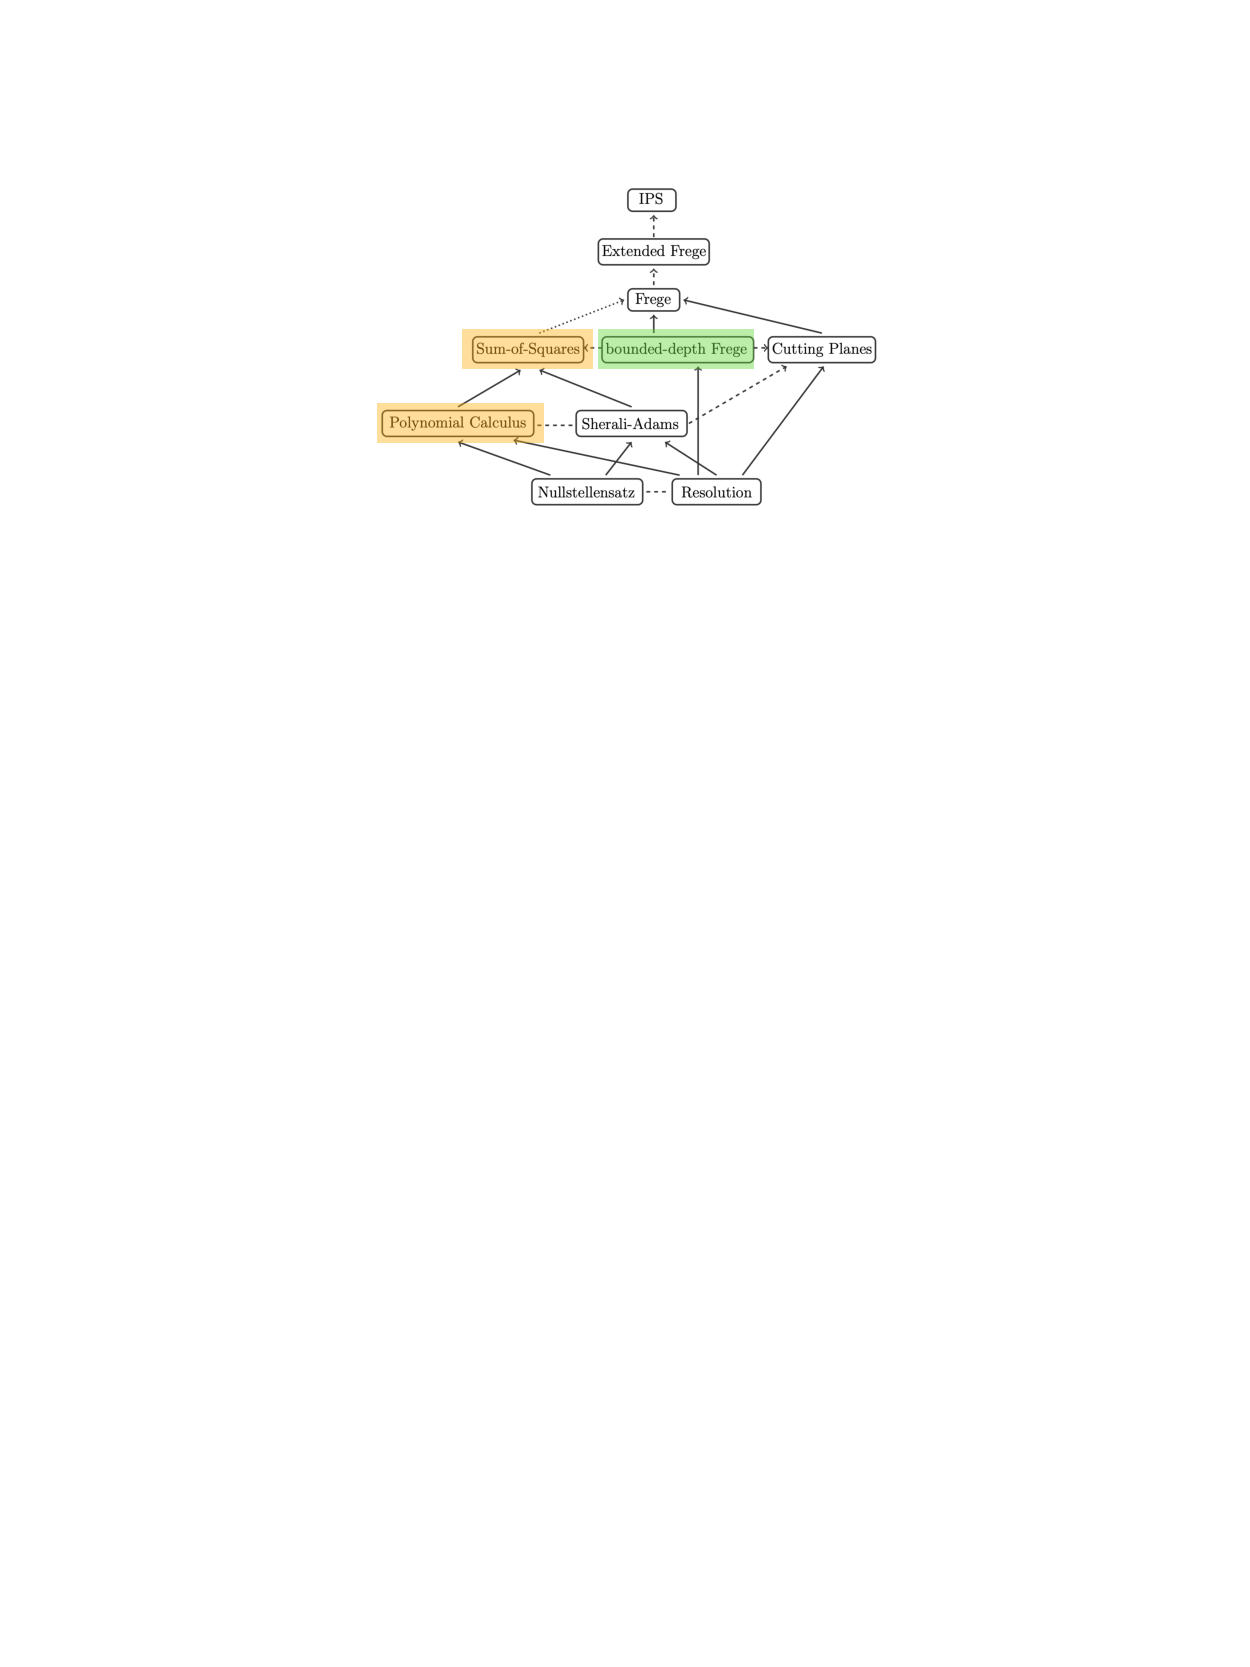
\includegraphics{assets/proof-system-relationships.pdf}
	\caption{The figure above (sourced from \citep[Page 10]{ProofComplexityLecNotes}) depicts proof systems commonly studied by the community and how they relate to each other.}
	\label{fig:example-proof-systems}
\end{figure}

In their seminal work, \citet{cook1979relative} introduced a program for separating $\CoNP$ from $\NP$.
Given a propositional formula $\PropFormula$, the task is to study the complexity of proofs for the claim \textit{``that $\PropFormula$ is unsatisfiable''}.
Showing that there exists no short\footnote{By short we mean polynomial in the size of the instance.} proofs for unsatisfiability would imply $\CoNP \neq \NP$, which would further imply $\P \neq \NP$, resolving one of the most fundamental open problems in computer science and mathematics.
With no other restrictions for the language with which we describe a proof, we are currently do not possess the tools to show lower bounds for general proof systems. 
However still, it is widely conjectured that $\CoNP \neq \NP$, and thus, as an intermediate step towards making partial progress, the research community has invested a significant amount of time and energy in proving size lower bounds for more restricted proof systems \citep{blake1937canonical,razborov1998lower, impagliazzo1999lower, alekhnovich2001lower, buss1999linear}.
When we say restricted proof system, we mean there is a fixed set of axioms and inference rules, and a restriction on the language that can be used to write down lines of the proof. We refer the reader to \citep{krajicek2019proof} for detailed introduction to the formalities of describing a proof system.
A simple example of a proof system is that of truth tables i.e. given a formula $\PropFormula$, a valid proof is simply the truth table for the formula.
For such a proof system, given a formula on $n$ variables, the size of the proof is $2^n$ and it is easy to see that we cannot use shorter proofs.
However, truth tables are very from being general proof systems, and to make progress towards the final goal, the research community has considered increasingly more expressive proof systems such as resolution, bounded depth Frege proof systems, Nullstellensatz etc.
Figure \ref{fig:example-proof-systems} lists some these proof systems and describes the relationships between them.
We refer the reader to \citep{krajicek2019proof, ProofComplexityLecNotesPaul} for more details on the definitions of the various proof systems.
Proof systems listed at the top of Figure \ref{fig:example-proof-systems} are more expressive\footnote{Expressiveness is formalised by the notion of $p$-simulation, and we refer the reader to \citep[Definition 1.6]{ProofComplexityLecNotes} for more details.}, and lower bounds for such proof systems subsume claims about the complexity of proofs lower in the figure.\par
In this work, we focus on the semi-algebraic proof systems of polynomial calculus (PC) \citep{alekhnovich2004pseudorandom} and sum of squares (SOS) \citep{parrilo2000structured, boazCourse}.
In a semi-algebraic proof system like PC and SOS, instead of a propositional formula over $n$ variables, we are given a set $Q=\{q_i(\vec{x}) \text{ } |\text{ } i \in [m] \}$ of polynomial equations over $n$ variables $\vec{x} = (x_1, \dots, x_n)$ as the problem instance.
In PC, the polynomials can be over \emph{any} field $\Field$, and in SOS, the polynomials must be over the reals.
We say a proof $\Proof$ is a refutation of $Q$, if it is a proof of the claim (in the specified language) that there exists no assignment of $\vec{x} \in \Field^n$ that satisfies \emph{all} the polynomial equations in $Q$. 
In PC and SOS, the proof $\Proof$ is itself expressed as polynomial.  
The size of a proof in the above systems is measured by the maximum of degree of the proof polynomial that refutes $Q$ (see Section \ref{sec:proof-system-prelims} for more details).
We denote the degree of such proof polynomials with $\Degree{Q \PC \bot}$ and $\Degree{Q \SOS \bot}$ for PC and SOS respectively, and  main goal of the discipline to study how complexity of the degree of refutals for different constraints $Q$.
Often one can use semi-algebraic proof systems to capture constraints of combinatorial objects like graphs.
More specifically, given an undirected graph $G=(V,E)$, and a vector $\vec{b} = (b_1, \dots, b_{|V|})  \in \Field^{\Size{V}}$, we define $\Card{G, \vec{b}}$ as the following set of polynomial constraints over variables $x_1, \dots, x_{|E|} \in \Field^{\Size{E}}$

\begin{definition}[Card]\label{def:card}Given a graph $G=(V,E)$, and a vector of constants $\vec{b} = (b_1, \dots, b_{|V|}) \in \Field^{|V|}$,

\begin{displaymath}
        \Card{G, \vec{b}}=
        \Bigger[10]\{\begin{array}{@{}cl}
                x_{\highlight{e}}(1 - x_{\highlight{e}}) = 0 & \text{ for every $\highlight{e} \in E$}\\[3mm]
                \underset{e \in E}{\sum x_e}= b_{\highlight{v}} & \text{ for every $\highlight{v} \in V$} \\[3mm]
        \end{array}
\end{displaymath}
	
\end{definition}

For every $e \in E$, if the polynomial equation $x_e(1 - x_e) = 0$ were to be satisfied, then it restricts the domain of the above variables to bits i.e. $x_e \in \bit$ for all $e \in E$.
Note if there was an assignment of variables in $\vec{x} \in \bit^{|E|}$ that satisfied all the equations in $\Card{G, 1^{|V|}}$, it would imply that the graph $G$ has a perfect matching (given by the edges corresponding to variables with assignment 1).  
When $|V|$ is odd, we know that any graph $G$ cannot have a perfect matching.
In other words, $\Card{G, 1^{|V|}}$ cannot be satisfied.
In this work we are interested in the complexity of PC and SOS refutations for $\Card{G, 1^{|V|}}$  when $|V|$ is odd.
With no further constraints on $G$, we do not have general lower bounds on the proof sizes for these refutations.
In recent work \citep[Open Problem 7.7]{buss2021proof}, Buss and Nordstr{\"o}m asked ``\textit{Are even colouring formulas over expander graphs hard for
polynomial calculus over fields of characteristic distinct from 2 ?}''
The even colouring formula is a special case of $\Card{G, \vec{b}}$, where each coordinate  $\vec{b}$ is $\degree{G}{v}/2$ for $v \in V$.
Therefore, their open question can be reformulated as the following question.

\begin{boxedproblem}
Do refutations for $\Card{G, \vec{b}}$ for
polynomial calculus over fields of characteristic $\neq 2$ have large size, when $G$ is an expander graph?
\end{boxedproblem}

\citet{Austrin_2022} made partial progress on the above problem by showing that the perfect matching principle requires large size on \highlight{random $d$-regular graphs} (for some constant $d$) in the Sum-of-Squares and Polynomial Calculus proof systems.
More formally, they show that 

\begin{theorem}{\citep{Austrin_2022}}{thm:prev-thm}
There is a constant $d_0 \in \Naturals$ such that for all $d \geq d_0$, and $\vec{b} \in [d]^{\Size{V}}$, the following holds asymptotically almost surely over a random $d$-regular graph $G=(V,E)$ on $n$ vertices:
\begin{enumerate}
    \item{ $\Degree{\Card{G, \vec{b}} \PC \bot} = \BigOmega{\frac{n}{\log n}}$} 
    \item{$\Degree{\Card{G, \vec{b}} \SOS \bot} = \BigOmega{\frac{n}{\log n}}$}
\end{enumerate}
\end{theorem}

Given a random $d$-regular graph $G$ on $n$ vertices, the authors start with the worst case hard graph $H$ described by \citet{buss1999linear}.
Such a graph is known to have $\Degree{\PerfectMatching{G} \PC \bot} = \BigOmega{\Size{V(H)}}$ (see \citep[Appendix A]{Austrin_2022} for details about how $H$ is constructed and \citet{buss1999linear} for hardness proof).
The main task then is to \emph{embed} $H$ into $G$ in such a way that that the hardness of $H$ is transferred to $G$.
One of the features of the embedding theorem above is that the embedding must be random \citep[See Section 6]{Austrin_2022}.

\paragraph{Our Contribution} In this work, we improve upon the result by \citet{Austrin_2022}, and directly answer Buss and Nordstr{\"o}m's question. 
We show that refutations for $\Card{G, \vec{b}}$ have large size for Sum-of-Squares and Polynomial Calculus for expander graphs.
Note that, we prove lower bounds for a larger class of graphs, that includes random $d$-regular graphs as a subset.
Our main result is stated below.

\begin{theorem}{Main Result}{thm:main-thm}
There is a constant $d_0 \in \Naturals$ such that for all $d \geq d_0$, the following holds asymptotically almost surely for any $(n, d, \lambda)$-graph $G$ on $n$ vertices, where $n$ is odd and $\lambda < ??$:
\begin{enumerate}
    \item{ $\Degree{\PerfectMatching{G} \PC \bot} = \BigOmega{\nicefrac{n}{\log n}}$} 
    \item{$\Degree{\PerfectMatching{G} \SOS \bot} = \BigOmega{\nicefrac{n}{\log n}}$}
\end{enumerate}

\ari{Re-write all the constants in this theorem, once we've vetted all the proofs}.

\end{theorem}


Our result also follows the general technique used in \citep{Austrin_2022} with notable differences.

\ari{How are we different, and give a bit more clarity on this.}
However, our results differ in the following significant way 
(1) Our embedding techniques make no use of randomness as they need to work for $\EnDeeLambda$ graphs (which can be deterministic constructions).



\section{Technical Overview}

Put in proof by pictures here.



\section{Preliminaries}

\paragraph{Notation} Sets are denoted with upper case normal font e.g., $S$. Families (or collections) of sets are denoted with upper case calligraphic purple text e.g., $\Family{S}$. 


\begin{definition}[Dependency Graphs]\label{def:dep-graphs}
	
\end{definition}

\begin{lemma}[Lov\`asz Local Lemma]\label{lemma:lll}Let $\Dist \in \DistSet{\bit^*}$ be a discrete probability distribution.
Let $E_1,...,E_n$ be a set of events, and assume that the following hold: (1) The degree of the dependency graph given by $(E_1, \dots, E_n)$ is bounded by $d$, and (2) $\PProb{E_i}{\Dist} \leq \beta$ for some $\beta \leq \frac{1}{4d}$. Then,

\[ \PProb{\overset{n}{ \underset{i=1}{\cap}} \hspace{0.1cm}  \overline{E_i}}{\Dist} > 0\]	
	
\end{lemma}

\subsection{Proof Complexity Preliminaries}
\label{sec:proof-system-prelims}
\begin{definition}[Polynomial Calculus Refutations]\label{def:poly-calc-refutations}
	
\end{definition}

\subsection{Graph Theory Preliminaries}

For a graph $\Graph$, we use $\Vertices{\Graph}$ and $\Edges{\Graph}$ to denote the vertices and edges of $\Graph$. 
For any $E' \subseteq \Edges{\Graph}$ and a vertex $v \in \Vertices{\Graph}$, we use $\Neighbourhood{E'}{v} = \{ u \in \Vertices{\Graph} : (u,v) \in E' \}$ to denote the neighbourhood of $v$ with respect to $E'$, and $\degree{E'}{v}$ to denote the number of vertices adjacent to $v$ via edges in $E'$.

\begin{definition}[Subgraph]\label{def:subgraph}
A graph $G'=(V', E')$ is a subgraph of another graph $G=(V, E)$ iff (1) $V'\subseteq V$, and (2) $E'\subseteq E$ and  $(v1, v2) \in E' \implies (v1, v2) \in V')$.
	
\end{definition}

\begin{definition}[Sub-divisions]\label{def:subdivisions}
Given a graph $H$ and a function $\sigma: \Edges{H} \rightarrow \Naturals$, the $\sigma$-subdivision $H$, denoted by $\Subdivision{H}{\sigma}$, is the graph obtained by replacing each edge in $\Edges{H}$ with a path of length $\sigma(e)$ joining the end points of $e$ (such that all these paths are mutually vertex disjoint, except at the end points).	
\end{definition}

\begin{definition}[Topological Minor]\label{def:topological-minor}
A graph $H$ is a topological minor of a graph $G$ if there exists a subdivision $\Subdivision{H}{\sigma}$ that is isomorphic to \emph{any} subgraph of $G$.	
\end{definition}

Next we define pseudorandom graphs or expander graphs. 
Throughout this document, it suffices to treat $d$ as a small constant.

\begin{definition}[$\EnDeeLambda$ pseudorandom graphs]\label{def:expander-graphs}
Let $G$ be a $d$-regular graph on $n$ vertices, and, let $\lambda_1 \geq \lambda_2, \dots, \geq \lambda_n$ denote eigenvalues of the adjacency matrix of $G$.
We say $G$ is an $\EnDeeLambda$-graph if $\ExpansionFactor{\Graph} \Def \underset{{\{2, \dots, n\}}}{\max}|\lambda_i| \leq \lambda$.
\end{definition}


\begin{lemma}[Expander Mixing Lemma]\label{lemma:expanders-mixing-lemma}
	
\end{lemma}


\section{Embedding Machinery}

The following definitions are adapted from \citep{nenadov2023routing} but were originally introduced by \citet{feldman1988wide} in their work about the theory of wide sense blocking networks.

\begin{definition}[$(p, q)$-non blocking bipartite graphs \citep{nenadov2023routing}]
Given $p,q \in \Naturals$ , we say that a bipartite graph $\Graph = (A \cup B, E)$ is $(p, q)$ \emph{non-blocking}, if there exists a family $\Family{S}$ of subsets of $E$, called the \emph{safe states}, such that the following holds:

\begin{enumerate}
	\item $\emptyset \in \Family{S}$
	\item If $E'' \subseteq E'$ and $E' \in \Family{S}$, \emph{then}, $E'' \in \Family{S}$.
	\item Given $E' \in \Family{S}$ such that $|E'| \leq p$, and \emph{any} $v \in A$ with $\degree{E'}{v} < q$, there exists $e = (v, w) \in E \setminus E'$  such that (i) $E' \cup \Set{e} \in \SafeStates $, and (ii) $w$ is not incident to any edge in $E'$ i.e. $\forall x \in A$ we have $(x,w) \notin E'$. 
 We call $w$ a \emph{safe neighbour} for $v$ given $E'$.
\end{enumerate}

\end{definition}


\paragraph{Why are non-blocking graphs useful} 
\ari{Use the get out of jail analysis I wrote down.}\par
\begin{figure}[h]
\center
{\caption{A test figure with its caption side by side}\label{fig:test}}
{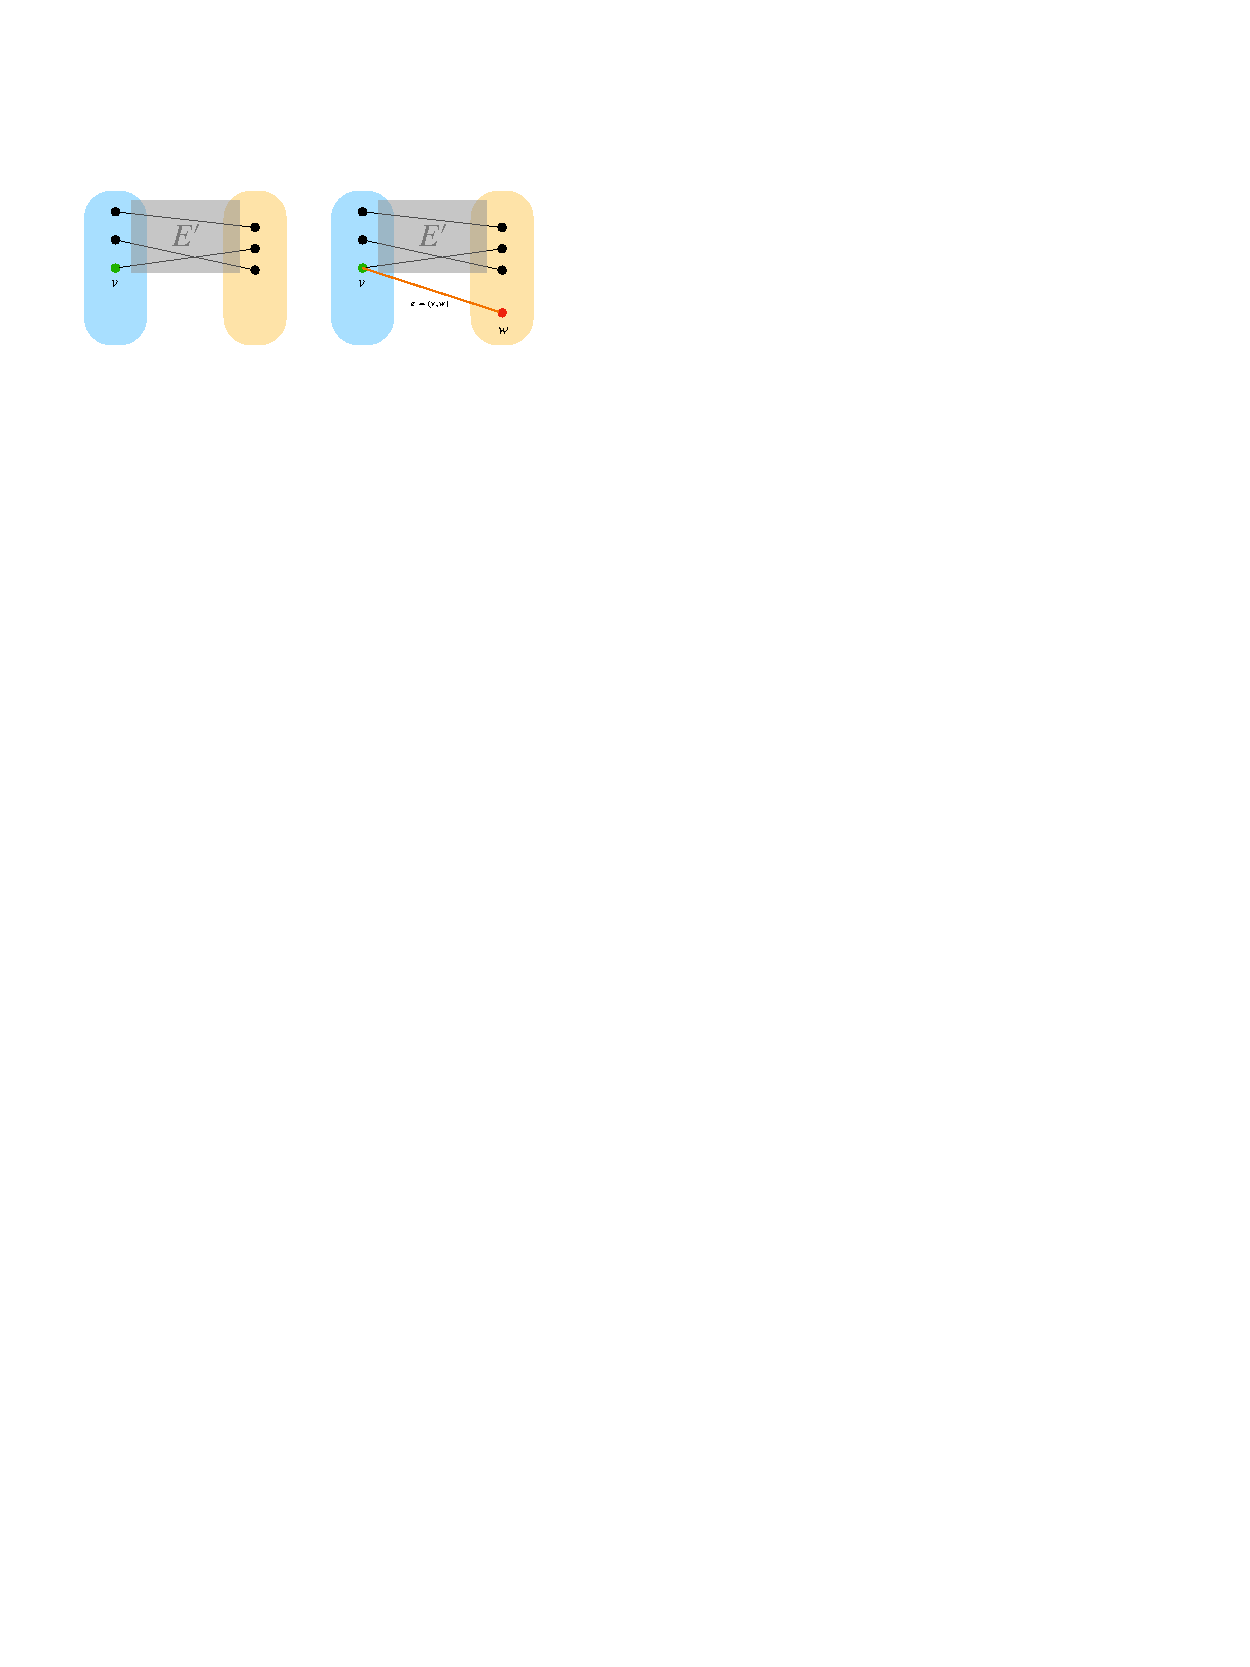
\includegraphics{assets/non-blocking-networks.pdf}}
\end{figure}

Next, we re-state a lemma by \citep[Proposition 1]{feldman1988wide} which describes the properties bipartite graphs must satisfy to be non-blocking.

\begin{lemma}\label{lemma:condtions-for-non-block}
Fix $a, r, s \in \Naturals$. Let $\Graph = (A \cup B, E)$ be a bipartite graph.
If for every $X \subseteq A$ of size $1 \leq |X| \leq 2a$, there are \emph{at least} $(r + s)|X|$ vertices in $B$ that are adjacent to $A$, \emph{then}, $\Graph$ is $(r, as)$-non blocking.
\end{lemma}


\section{Proof Of Main Result}

Let $G=(V,E)$ denote any $\EnDeeLambda$-graph on an odd number of vertices, and,  $\HardInstance$ denote the hard instance on $t$ vertices for polynomial calculus, as described by \citet{buss1999linear}, where the refutal certificate is of degree $\BigOmega{t}$.
The hardness proof follows from the following steps:


\begin{enumerate}
	\item First, we show (via the \nameref{theorem:partition}) that we can partition the vertices of the graph $\Graph$ into two disjoint sets $A$ and $B$, as shown in Figure \ref{subfig:partitionA}. The partition has the property that for each vertex $v \in V$, $\Eps'd \leq |\Neighbourhood{E}{v} \cap A| \leq \Eps d$, where $0 <\Eps '< \Eps < 1$ are small constants. Given this partitioning, we define consider the subgraph $G_A = (A, E_A)$ where we only include edges with both endpoints in $A$ (see Figure \ref{subfig:partitionB}).
	\item Let $D = d/\ExpansionFactor{G}$. We find a subdivision $\Subdivision{H}{\sigma}$ of $H$, where for each $e \in \Edges{H}$, we have $\sigma(e) = \PathSize$, where $\PathSize = 2k+1$ is an odd integer for $k = \BigO{\log_{D} n}$. We show (via the \nameref{theorem:top-embedding}) that $\Subdivision{H}{\sigma}$ is a subgraph of $G_A$ defined above. \ari{Add in the alternating argument.}
	
%	\item Successfully executing the above steps guarantees that $\HardInstance$ exists inside of $\Graph$ as a topological minor. But as described earlier, this does not suffice in showing that $\PerfectMatching{\Graph}$ is also hard to refute. Let $\Embedding{\HardInstance}$ denote the vertices that form the topological embedding of $\HardInstance$ in $\Graph$. We want to show that the induced subgraph $\Graph[\Vertices{\Graph} \setminus \Embedding{\HardInstance}]$ contains a perfect matching. 
	\item We show (via the \nameref{theorem:perfect-matching}) that the subgraph of $G$ not participating in the topological embedding above, has a perfect matching $M$. For all $e \in M$, we set $x_e = 1$ and for all $e \notin \Edges{\Embedding{\Subdivision{H}{\sigma}}}$ but not in $M$, set $x_e = 0$. These assignments imply that the formula for refuting $\PerfectMatching{G}$ can be partially filled up, and we are left with the task of refuting a restricted formula. Refuting this restricted formula is identical to finding a refutation in the original hard instance, and thus the proof complexity for refuting perfect matching for $G$ is $\BigOmega{t}$ where $t$ is the number of vertices in the hard instance $H$. We show that $t = \BigOmega{n\log n}$.
\end{enumerate}

\subsection{Step 1: Partition $G$ into $A$ and $B$}

\begin{lemma}[Multiplicative Chernoff Bound]\label{lemma:mult-chernoff}
Suppose $X_1, ..., X_n$ are identical independent random variables taking values in $\{0, 1\}$. Let $X$ denote their sum and let $\mu = n\Mean{}{X_1}$ denote the sum's expected value. Then for any $0 < \delta < 1$

\[ \Prob{|X - \mu| \geq \delta \mu} \leq 2\exp(-\delta^2\mu/3)\]
	
\end{lemma}

%\begin{figure*}[t!]
%    \centering
%    \begin{subfigure}[t]{0.5\textwidth}
%        \centering
%        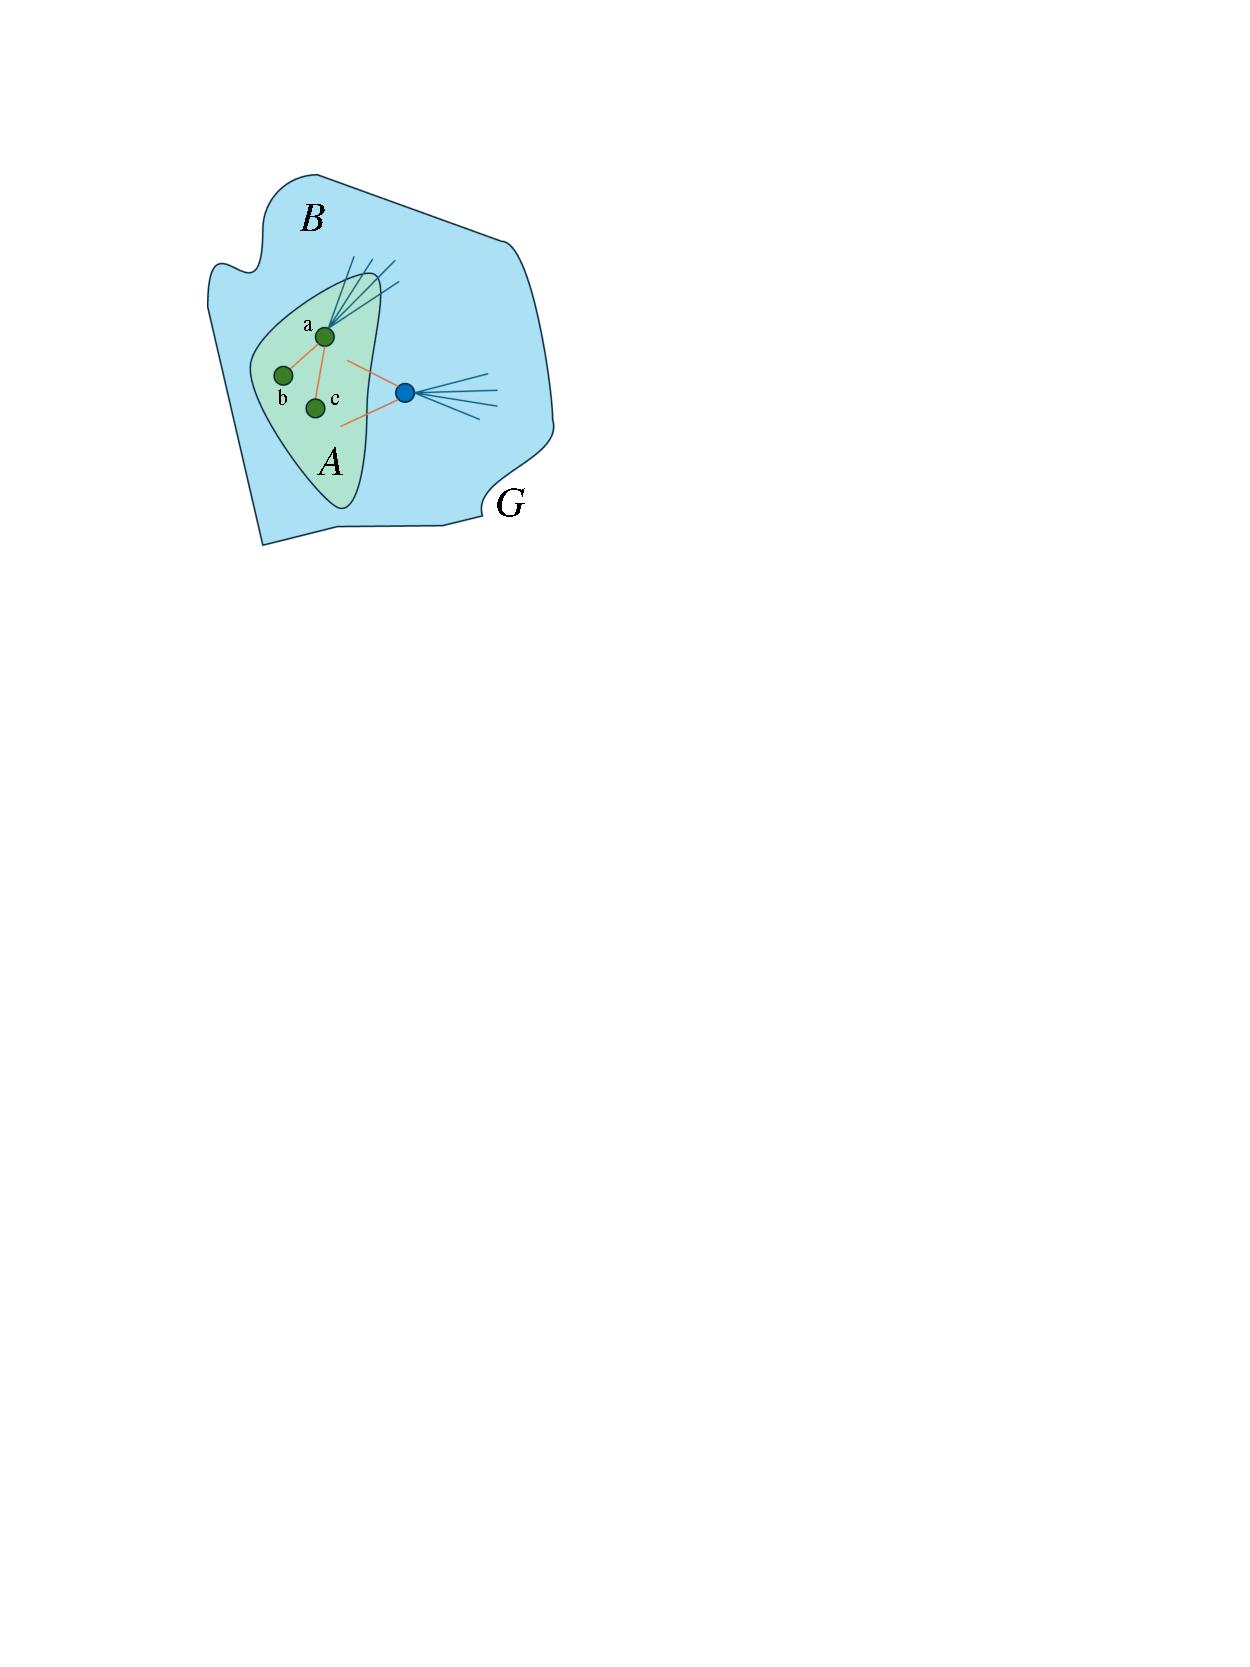
\includegraphics{assets/ParitionA.pdf}
%        \caption{The figure above describes the partitioning of the vertices of the graph $G$ into two sets $A$ and $B$, such that for every vertex $v \in \Vertices{G}$, $\epsilon d$ fraction of the edges go into $A$ (depicted in orange) and $1 - \epsilon d$ fraction of the edges go into $B$.}
%    \end{subfigure}%
%    ~ 
%    \begin{subfigure}[t]{0.5\textwidth}
%        \centering
%        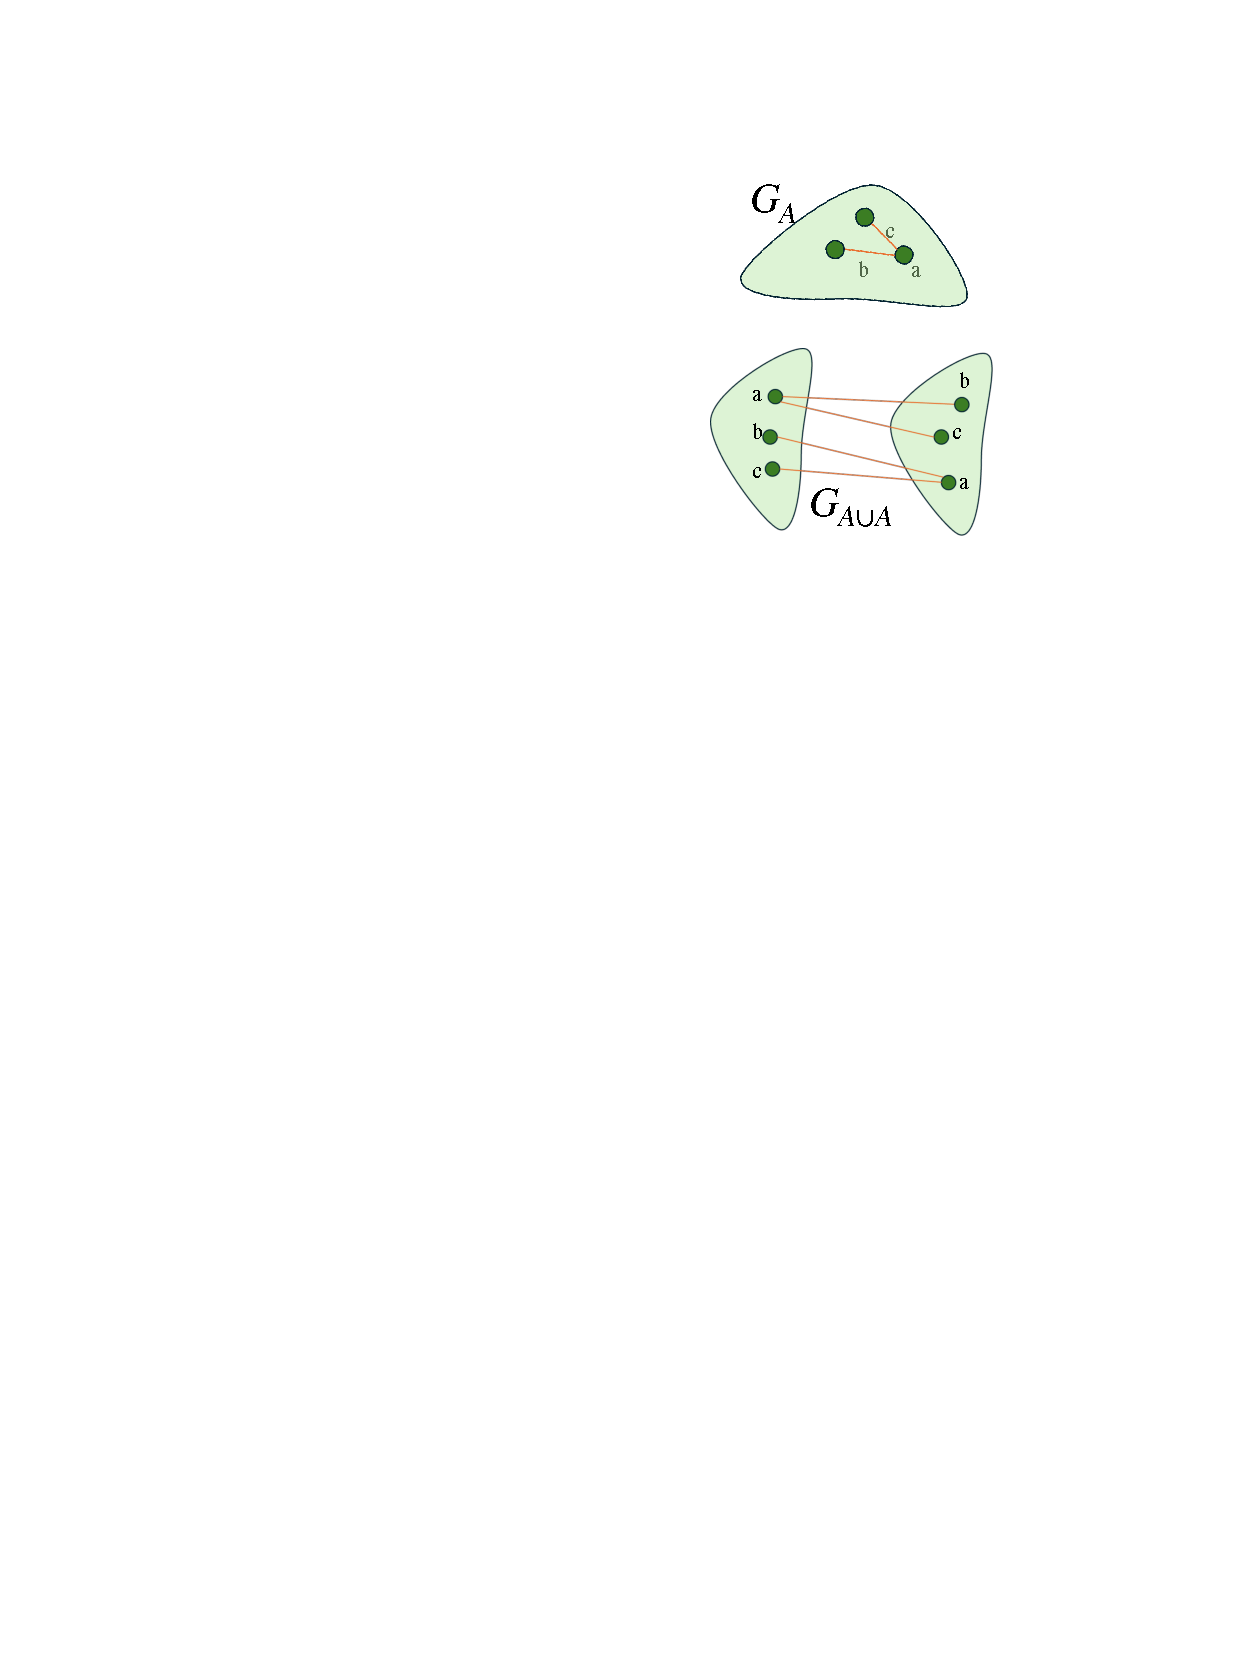
\includegraphics{assets/PartitionB.pdf}
%        \caption{The figures on top describes the subgraph $G_A$ obtained by including vertices in $A$, and only edges that stay inside $A$ (orange edges). The figure below describes how we construct a bipartite graph $\BipartiteG$ from $G_A$.}
%    \end{subfigure}
%%    \caption{Caption place holder}
%\end{figure*}

\begin{figure*}[t!]
    \centering
    \begin{subfigure}[t]{0.45\textwidth}
        \centering
        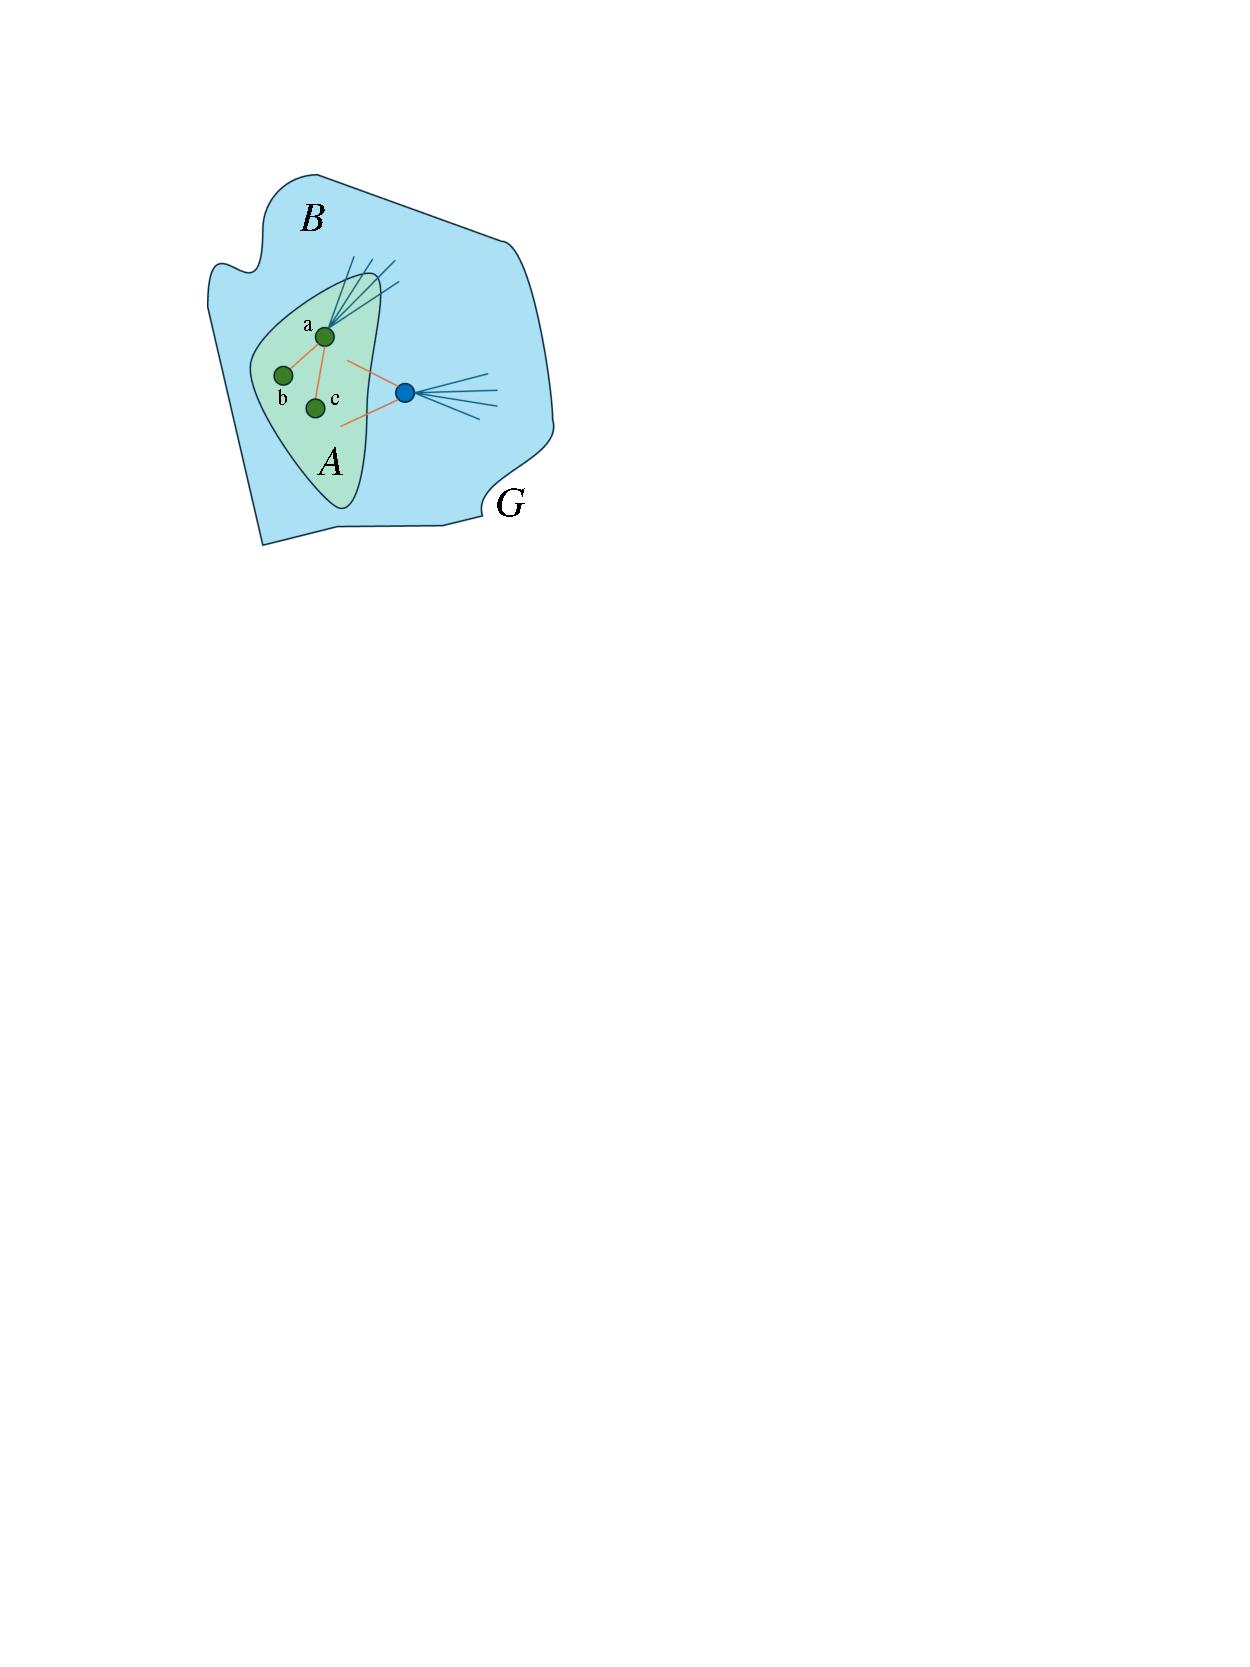
\includegraphics[width=0.8\textwidth]{assets/ParitionA.pdf}
        \caption{The figure above describes the partitioning of the vertices of the graph $G$ into two sets $A$ (highlighted in green) and $B$ (highlighted in blue), such that for every vertex $v \in \Vertices{G}$, $\epsilon d$ fraction of the edges go into $A$ (depicted in orange) and $1 - \epsilon d$ fraction of the edges go into $B$.}
        \label{subfig:partitionA}
    \end{subfigure}%
    \hspace{1mm}
    \vrule width 1pt % vertical line
    \hspace{1mm}
    \begin{subfigure}[t]{0.45\textwidth}
        \centering
        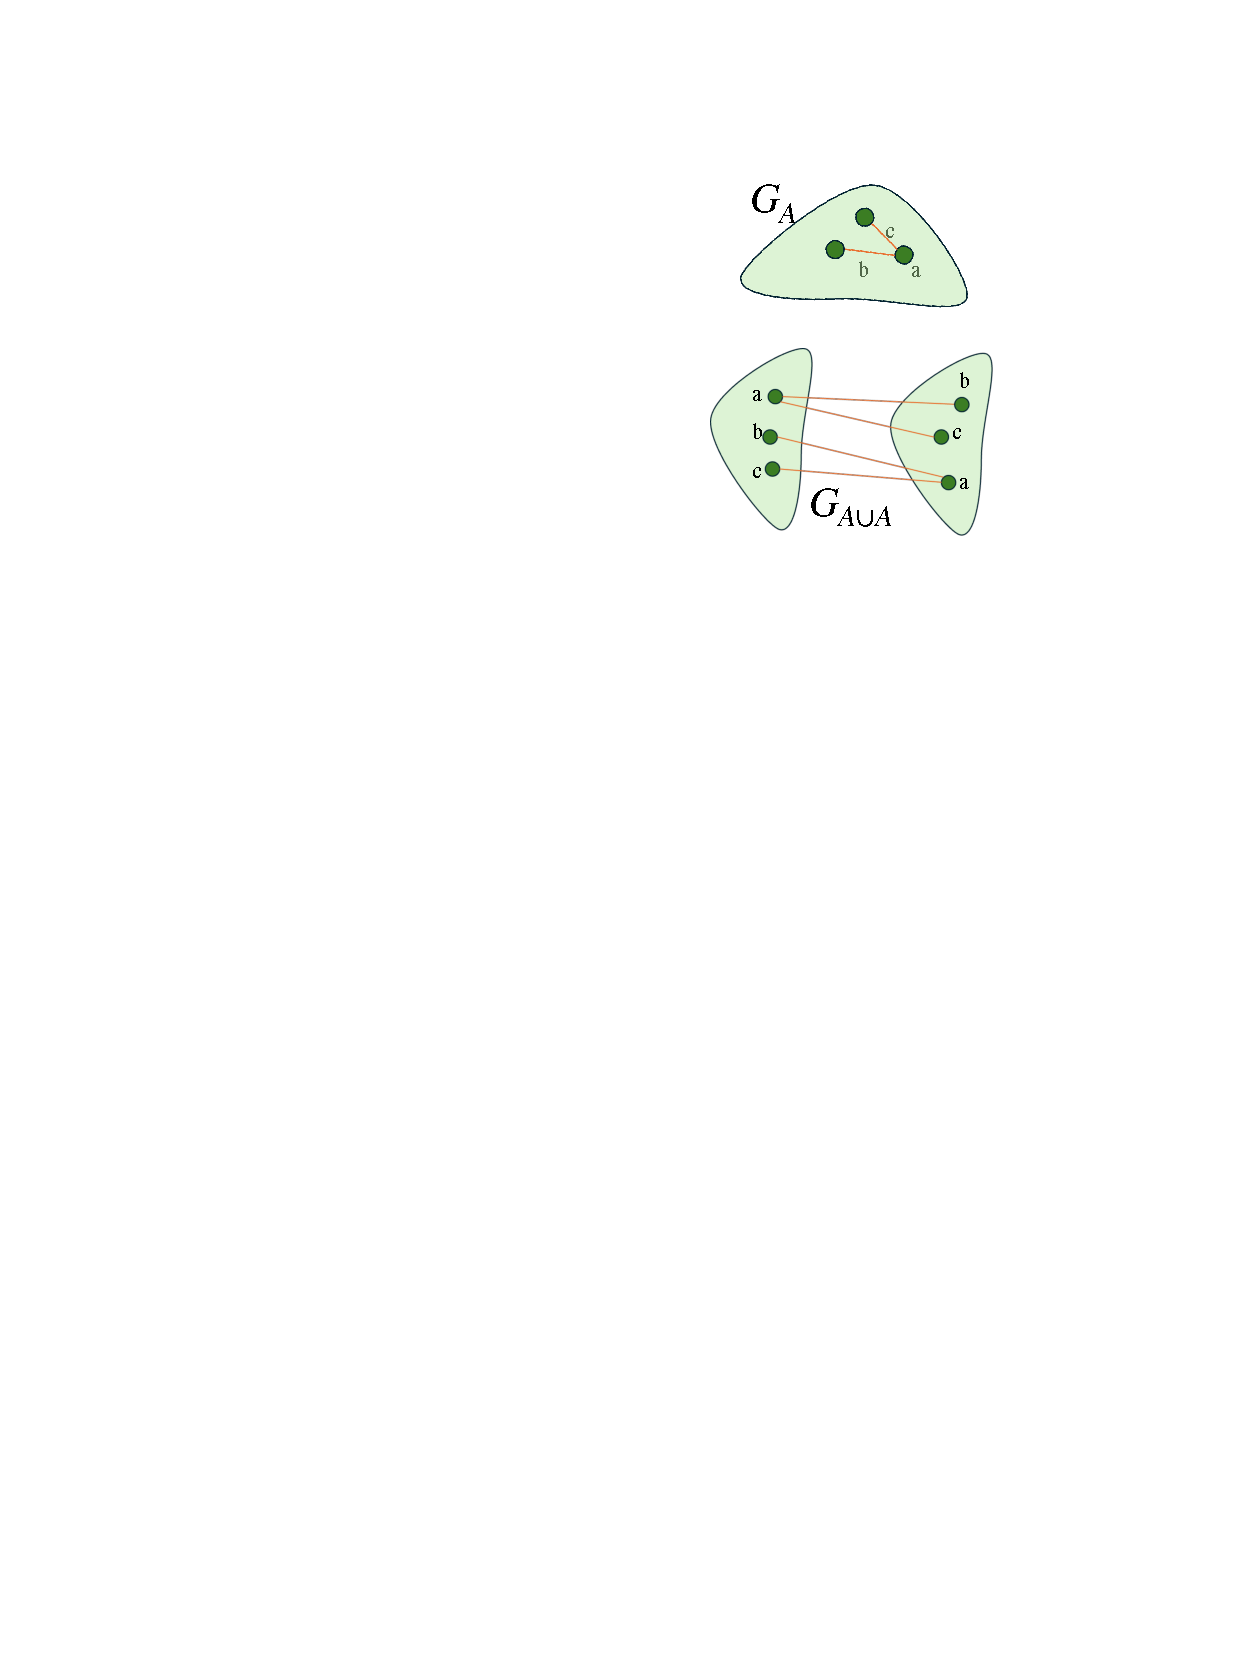
\includegraphics[width=0.8\textwidth]{assets/PartitionB.pdf}
        \caption{The figures on top describes the subgraph $G_A$ obtained by including vertices in $A$ and edges that stay inside $A$ (orange edges), as described in the construction of Step 2. The figure below describes the bipartite graph $\BipartiteG$ we use for the embedding theorem.}
        \label{subfig:partitionB}        
    \end{subfigure}
\end{figure*}


\begin{theorem}{Partition Theorem}{partition}
There exists a constant $d_0 \in \Naturals$ and small constants $\delta \in (0,1)$ such that, given a $\EnDeeLambda$ graph $\Graph = (V, E)$, with $d \in [d_0, n-1]$, there exists and a partition of $V$ into disjoint sets $A$ and $B$, such that, we have for every $v \in V$, $ \Eps'd \Def \alpha(1-\delta)d\leq |\Neighbourhood{\EdgesShort}{v} \cap A| \leq \alpha(1+\delta)d \Def \Eps d$ where $\alpha=0.1$ is a small constant.

	
\end{theorem}

\begin{proof}We prove the existence of such a partition $A \cup B = V$ using the probabilistic method.
For each $v \in \Vertices{\Graph}$, we toss an independent coin $X_i$ with bias $\alpha$.
If $X_i = 1$, then we include $v$ in $A$, else we put $v$ in $B$.
Thus, $\vec{X} \Def (X_1, \dots, X_n) \in \bit^n$ is a random variable that describes how we partition $V$ into sets $A$ and $B$.
For any $v \in V$, let $Y_v = |\Neighbourhood{\EdgesShort}{v} \cap A| = \sum_{x \in \Neighbourhood{E}{v}} \Indicator{x \in A}$ denote the random variable that counts how many neighbours of $v$ are also in $A$.\\
For any $\delta \in (0,1)$ and for any $v \in V$, let $E_v = \Indicator{|Y_v - d\alpha | \geq \delta \alpha d}$ denote the bad event that $Y_v$ is bounded away from $\alpha d$ by a multiplicative factor of $\delta$.
As $\Graph$ is $d$-regular, $\Mean{\vec{X}}{Y_v} = \alpha d$, and observe that the dependency graph (Definition \ref{def:dep-graphs}) of events $\{ E_v \}_{v \in V}$ has max-degree at most $d$.
By the multiplicative Chernoff bound (Lemma \ref{lemma:mult-chernoff}), for any $v \in V$, we have $\PProb{E_v}{\vec{X}} \leq 2\exp(-\delta^2\alpha d/3) \Def \beta$.
For large enough $d$ i.e $d > d_0$, for some $d_0$, we can make $\delta \in (0,1)$ large enough, such that $2\exp(-\delta^2\alpha d/3) \leq 1/(4d)$. Therefore, we have $\beta d \leq 1/4$.
Thus, we can invoke the Lov\`asz Local Lemma (Lemma \ref{lemma:lll}) to get $\PProb{\forall v \in V, \text{ } E_v = 0}{\vec{X}} > 0$

\end{proof}

%Let $\tilde{\Graph} = A \cup B$ be the bipartite graph defined in the construction of Lemma \ref{lemma: bipartite-construct-non-block}.
%We know that this graph $(\pee, \qu)$ is non-blocking.
%Let $(a_1, \dots, a_k)$ denote an arbitrary ordering of arbitrary vertices in $A$.
%Set $E' = \emptyset$. 
%As $\tilde{\Graph}$ is non-blocking, there exists a collection of \emph{safe states} $\SafeStates$.


\subsection{Step 2: The Topological Embedding}

\ari{Revisit this again.}
Given $\EnDeeLambda$ graph $G=(V,E)$, let $A$ and $B$ be the partition guaranteed by the \ \nameref{theorem:partition}.
We also have that for all $v \in A$,  $|\Neighbourhood{\EdgesShort}{v} \cap A| \leq d \alpha(1+\delta) = \Eps d$, where $\Eps = (1+ \delta)\alpha$ and $\alpha, \delta \in (0,1)$ are constants as defined in the \nameref{theorem:partition}.
Define $\dApproxLower \Def \Eps d$.
Define $E_A \Def \{ (u,v) \in E : u \in A \land v \in A\}$. 
That is $E_A$ are the edges whose endpoints are fully contained in A (orange edges in Figure \ref{subfig:partitionA}), and $G_A = (A, E_A)$. 
Define $ \na = |A|$.
Now define a bipartite graph $\BipartiteG = (V_A \cup V_A)$ such that if $(u,v) \in E_A$, then $(u,v) \in \Edges{\BipartiteG}$.

\begin{lemma}\label{lemma:bipartitie-is-non-blocking}Let $G$ be the $\EnDeeLambda$ graph given to us and let $\BipartiteG$ be the bipartite graph described above. 
There exists $\epsilonL, \epsilonA  \in (0,1)$ small enough, such that if $\lambda < \epsilonL d$, then $\BipartiteG$ is $(\frac{d}{\lambda}, \epsilonA n)$ non-blocking.
\end{lemma}

\begin{proof}
Let $\BipartiteG = (X \cup Y, E_A)$. 
Let $\lambda = \ExpansionFactor{G} \leq d/c_2$ where $c_2 > 0$ is a constant to be defined later.
Set $a = \frac{n\lambda}{2c_1 d}$ for a constant $c_1 > 0$ to be defined later.
Set $c_1, c_2$ such that $\left(\frac{1}{c_1/2}  + \sqrt{\frac{1}{c_2/2}}\right) \leq \EpsLower$, where $\EpsLower$ is as defined in the \nameref{theorem:partition}.
Pick any $S \subseteq X$ with $|S| \leq 2a = \frac{n\lambda}{c_1 d}$.
\highlight{Assume towards a contradiction, that there exists a set $T \subseteq Y$, such that 
$\CutEdges{S}{T}{E_A} < 2|S|\frac{d}{\lambda}$.} 
By how we constructed $\BipartiteG$, we know that
\[ \CutEdges{S}{T}{E_A} \geq \EpsLower d.\]

However, $S$ and $T$ are also subsets of $\Vertices{G}$ and $G$ is a $\EnDeeLambda$ graph.
From the \nameref{lemma:expanders-mixing-lemma}, we have

\begin{align}
	\CutEdges{S}{T}{E_A} &\leq \frac{d}{n}|S||T| + \lambda\sqrt{|S||T|} \\
	&< 2\frac{2d^2}{n\lambda}|S|^2 + |S|\sqrt{2\lambda d} \label{eq:assumption}\\
	&\leq |S|\left(\frac{2d^2}{\lambda n} \frac{n\lambda}{c_1 d} + \sqrt{d\cdot \frac{d}{c_2/2}}\right) \label{eq:assumption-lambda}\\
	&= |S|d\left(\frac{1}{c_1/2}  + \sqrt{\frac{1}{c_2/2}}\right) \\
	&\leq |S|d\EpsLower \label{eq:constants}
\end{align}


\eqref{eq:constants} is a contradiction, so our \highlight{assumption} must have been wrong.
\eqref{eq:assumption} comes from our \highlight{assumption}.
\eqref{eq:assumption-lambda} comes from our assumption that $\lambda \leq d/c_2$ and $|S| \leq \frac{n\lambda}{c_1 d}$.
Finally we get our theorem statement by setting $\epsilonL = 1/c_2$ and $\epsilonA = 1/c_1$.

%Let $X$ and $Y$ denote the left and right vertices of the bipartite graph $\BipartiteG$.
%Define $a = \epsilonA\cdot\frac{\lambda \na}{\dApproxLower}$.
%Fix $S \subseteq X$ such that $1 \leq |S| \leq 2a$.
%Suppose towards a contradiction, $G_A$ is \emph{not} non-blocking.
%Then by Lemma \ref{lemma:condtions-for-non-block}, for all $T \subseteq Y$, $\EdgesAccross{S, T}{E_A} \leq (2\dApproxLower/\lambda)|S|$.
%Pick $T^* \subseteq Y$ such that 
%
%\begin{equation}
%\EdgesAccross{S, T^*}{E_A} \geq |S|\dApproxLower	 \label{eq:lots-edges}
%\end{equation}
%
%We know $T^*$ exists as $G_A$ is $\dApproxLower$ regular.
%From the expander mixing lemma \ref{lemma:expanders-mixing-lemma},
%
%\begin{align}
%	\EdgesAccross{S, T^*}{E_A} &\leq \frac{\dApproxLower}{\na}|S||T^*| + \lambda\sqrt{|S||T^*|} \\
%	&\leq \frac{\dApproxLower^2}{\na \lambda}|S|^2 + |S|\sqrt{2\lambda \dApproxLower} \label{eq:stepa}\\
%	&< \frac{\dApproxLower^2}{\na \lambda}|S|^2 + |S|\dApproxLower\sqrt{2\epsilonL } \label{eq:stepb}\\
%	&\leq |S|\dApproxLower\left[ \frac{\dApproxLower|S|}{\na\lambda} + \sqrt{2\epsilonL}\right] \\
%	&\leq |S|\dApproxLower\left[ \frac{\epsilonA}{2} + \sqrt{2\epsilonL}\right] \label{eq:stepc}
%\end{align}
%
%
%For Equation \eqref{eq:stepa} We use that $\EdgesAccross{S, T^*}{E_A} \leq (2\dApproxLower/\lambda)|S|$. For Equation \eqref{eq:stepb} we use $\lambda < \epsilonL\dApproxLower$. For Equation \eqref{eq:stepc} we use $|S| \leq 2a$.
%Setting $\epsilonA$ and $\epsilonL$ small enough such that  $\frac{\epsilonA}{2} + \sqrt{2\epsilonL} < 1$, we get a contradiction with Equation \eqref{eq:lots-edges}.

\end{proof}


The next step is to topologically embed hard instance $H$ into the subgraph $G_A = (A, E_A)$.
Note for every edge in $E_A$, by our construction, we will have a corresponding edge in the bipartite graph $\BipartiteG$.

\begin{theorem}{Topological Embedding Theorem}{top-embedding}
Let $G$ be a $\EnDeeLambda$ graph, and $\BipartiteG$ be the construction defined above, where $|A| = \na$.
Let $\dApproxLower \Def \Eps d$, and $H$ be the worst case hard instance on $t = \lceil\epsilonA \frac{\na}{\log \na}\rceil$ vertices, where $0 < \epsilonL < \epsilonA <1$ are the constants from  Lemma \ref{lemma:bipartitie-is-non-blocking}.	
\ari{Define $\sigma$}.
If $\lambda \leq \frac{\epsilonL\dApproxLower}{\log_D[\na]}$, then $G$ contains $\Subdivision{H}{\sigma}$ as a subgraph.

\end{theorem}



\begin{proof}
Define $D = \frac{d}{\lambda}$ and $k \Def \lceil\log_D\na\rceil$.
Let $\{ h_1, \dots, h_t\}$ denote the vertices of $H$.
Let $\EmbeddingFunc: \Vertices{\Subdivision{H}{\sigma}} \rightarrow \Vertices{G_A}$ be the bijective mapping between the vertices of $\Subdivision{H}{\sigma}$, and the vertices of $G_A$, that defines our topological embedding.
Our first task is to find a unique $\Embedding{h} \in \Vertices{G_A}$ for each $h \in \Vertices{H}$.
Let $\{a_1, \dots, a_{t}\}$ be arbitrary set of $t$ vertices in $\Vertices{G_A}$.
We repeat the following process to obtain $\{ \Embedding{h_1}, \dots, \Embedding{h_t}\}$.
Let $X=\Vertices{G_A}$ and $Y=\Vertices{G_A}$ denote the left and right sides of the bipartite graph $\BipartiteG$ described above.
\ari{Add in some intuition as to why we need to do this}

\begin{figure*}[t!]
    \centering
    \begin{subfigure}[t]{0.95\textwidth}
        \centering
        \includegraphics{assets/embeddingA.pdf}
        \caption{The \textcolor{purple}{purple} edges represent the edges in $\cup_{i=1}^j (M_j \cup M_j')$, which we have already included.
        For any $v$ in $S_j \subseteq X$ (\textcolor{cadmiumgreen}{green vertex}) we ask for $D$ neighbours in $S_{j+1} \subseteq Y$ (shown with \textcolor{cadmiumgreen}{green} and \textcolor{carminepink}{pink} lines). 
        Of these $D$ edges, by the non-blocking property, we know that there will be at least one edge (in this case there are 3 such edges shown in \textcolor{carminepink}{pink}) such that the endpoints in $Y$ are not connected to any of the \textcolor{purple}{purple} edges. The \textcolor{cadmiumgreen}{green} dotted edges are connected to vertices that are already incident by one of the \textcolor{purple}{purple} edges, and so we cannot use them. We will add the \textcolor{carminepink}{pink} edges will be added to $M_j$.}
        \label{subfig:embeddingA}
    \end{subfigure}%
    \hspace{1mm}
%    \vrule width 1pt % vertical line
    \hspace{1mm}
    \begin{subfigure}[t]{0.95\textwidth}
        \centering
        \includegraphics[]{assets/embeddingB.pdf}
        \caption{We restrict the size of $M_j$ to be $\min\{t, |S_{j-1}|D\}$ edges. As $k = \log_{D}[\na]$, eventually, for some $j \leq k$, we get $t \leq |S_{j-1}|D$.
        In the above example $M_{j-1}$ has size $D|S_{j-2}|$ but $M_j$ has size $t$. 
        From then on for all $j \leq i \leq k$, $|M_i|= t$.
        Furthermore, for $j \leq i \leq k$,  each vertex in $S_i$ will be connected to exactly one vertex in $S_{i+1}$.
        }
        \label{subfig:embeddingB}        
    \end{subfigure}
\end{figure*}


\begin{itemize}
	\item Define $E' = \emptyset$ to begin with, and as $\BipartiteG$ is a $(D, \epsilonA n)$-non blocking bipartite graph (by Lemma \ref{lemma:bipartitie-is-non-blocking}), $E'$ is a \emph{safe} state.
	\item For $a_1 \in X$, we ask for $D$ neighbours in $Y$. By the non-blocking property, we can find a \emph{safe neighbour} $\tilde{h}_1 \in Y$ such that there is no edge in $E'$ is incident on $\tilde{h}_1$. We set $\Embedding{h_1} = \tilde{h}_1$ and update $E' = E'  \cup \{(a_1, \tilde{h}_1)\}$.
	\item We repeat this process for all $a \in \{a_2, \dots, a_t\}$. For the $j$'th step, As $|E'| = j \leq t < \epsilonA\na$, for each $a_j$ we can always find a \emph{safe neighbour} $\tilde{h}_j$ in $Y$ such that there is an edge from $a_j$ to $\tilde{h}_j$, and there is no other edge in $E'$ so far, that is incident on each $\tilde{h}_j$.
\end{itemize}

Once this phase is complete, we have mapped every vertex of $H$ to a vertex in $G_A$.
That is $\Embedding{h_i} = \tilde{h_i}$ for all $i \in [t]$.
The next step to show that for each $(u,v) \in \Edges{H}$, there is a vertex disjoint path of odd length $\PathSize = 2k+1$ between $\Embedding{u}$ and $\Embedding{v}$ in $G_A$.
Let $(e_1, \dots, e_m)$ be an arbitrary ordering of edges in $\Edges{H}$.
We prove the result by induction on $m$.

\paragraph{Base case} 

Let $e_1 = (u,v)$. Define sets $S_0 = \{\Embedding{u}\}$ and $S'_0 = \{ \Embedding{v}\}$, and set $M_0 = \emptyset$ and $M_0' = \emptyset$.
For each $z=1, \dots, k$, we will define edge sets $\{ M_j\}_{j \in [k]}$ and $ \{ M'_j\}_{j \in [k]}$, and vertex sets $\{ S_j\}_{j \in [k]}$ and $\{ S'_j\}_{j \in [k]}$ inductively as follows:

\begin{tcolorbox}
Fix $ 1 \leq z \leq k$, iteratively, let $M_z$ and $M'_z$ be the sets of $|S_z| \Def \min\{t, |S_{z-1}|D\}$ edges in $E_A$ incident to $S_{z-1}$ and $\S_{z-1}'$ respectively, such these edges are safe with respect to $\cup_{i=1}^{z} (M_i \cup M'_i)$.\\


More concretely, fix $1 \leq z \leq k$, and for each $v \in S_z \subseteq X$, we ask for $D$ neighbours in $S_{j+1} \subseteq Y$ via edges in $E_A$.
As $\BipartiteG$ is $(D, \epsilonA n)$ non-blocking, we know that at least one of these edges will be a safe edge connecting us to a safe neighbour in $S_{j+1}$, as long as $|\cup_{i=1}^{z} (M_i \cup M'_i)|$ is not too large.
Figure \ref{subfig:embeddingA} illustrates this.
Since $|M_i| \leq t$ and $|M_i'| \leq t$ for all $i \in [k]$, and $k = \log_D n$, we always have $\cup_{i=1}^{z} (M_i \cup M'_i)| \leq 2tk \leq \epsilonA n$.
If there are more than one safe edges for  vertices in $S_j$, consider at least one safe edge per vertex $v \in S_j$ to add to $M_j$ and, make sure $|M_j| = \min\{t, |S_{j-1}|D\}$.
Figure \ref{subfig:embeddingB} illustrates this idea.
$M'_j$ and $S_j'$ are constructed analogously.\\



\end{tcolorbox}

Let $M = \cup_{i=1}^k (M_i \cup M'_i)$.
The reason we can always construct the sets described above sets is that $|M| \leq tk < \epsilonA n$, and as $\BipartiteG$ is $(D, \epsilonA n)$ non-blocking, for any vertex $x \in S_j \subseteq X$, with at most $D$ neighbours in $S_{j+1} \subseteq Y$, we can always find \emph{at least} one $y \in S_{j+1}$, such that $(x,y) \in E_A$ and no edge in $\cup_{i=1}^{j-1} (M_i \cup M'_i)$ is incident on $y$.
Now as $k = \log_D[n]$, we have that, $|S_k| = |S_k'|= t$.
By the expander mixing lemma \ref{lemma:expanders-mixing-lemma},

\begin{align}
\CutEdges{S_k}{S_k'}{E_A}
 &\geq \frac{d t^2}{n} - \lambda t \\
	&> 0 \label{eq:greater}
\end{align}

Equation \eqref{eq:greater} comes from the assumption $\lambda \leq \epsilonL d$ (from Lemma \ref{lemma:bipartitie-is-non-blocking}).
This implies there exists at least one edge $e=(x,y)$ between $S_k$ and $S_k'$.
By how we constructed $M_k$, we know there is an edge $m_k = (a,x) \in M_k$ connecting $x$ to some vertex $a$ in $S_{k-1}$. 
Similarly, there is some edge $m_{k-1} \in M_{k-1}$ that connects $x$ to some vertex in $S_{k-2}$.
We repeat this process all the way, till we get $k+1$ edges, $m_1 m_2 \dots, m_k e$.
We repeat the same process for the other end point of $y \in S_k'$, to get edges $m'_1, \dots, m'_k$.
We add these edges to a global edge set $\GlobalEdgeSet$.
This gives is the situation depicted in Figure \ref{fig:baseB}.
Thus, we have found an odd length path $m_1\dots m_k e m_1'\dots m_k'$ of length $2k+1$, connecting $\Embedding{u}$ to $\Embedding{v}$.

\begin{figure}
	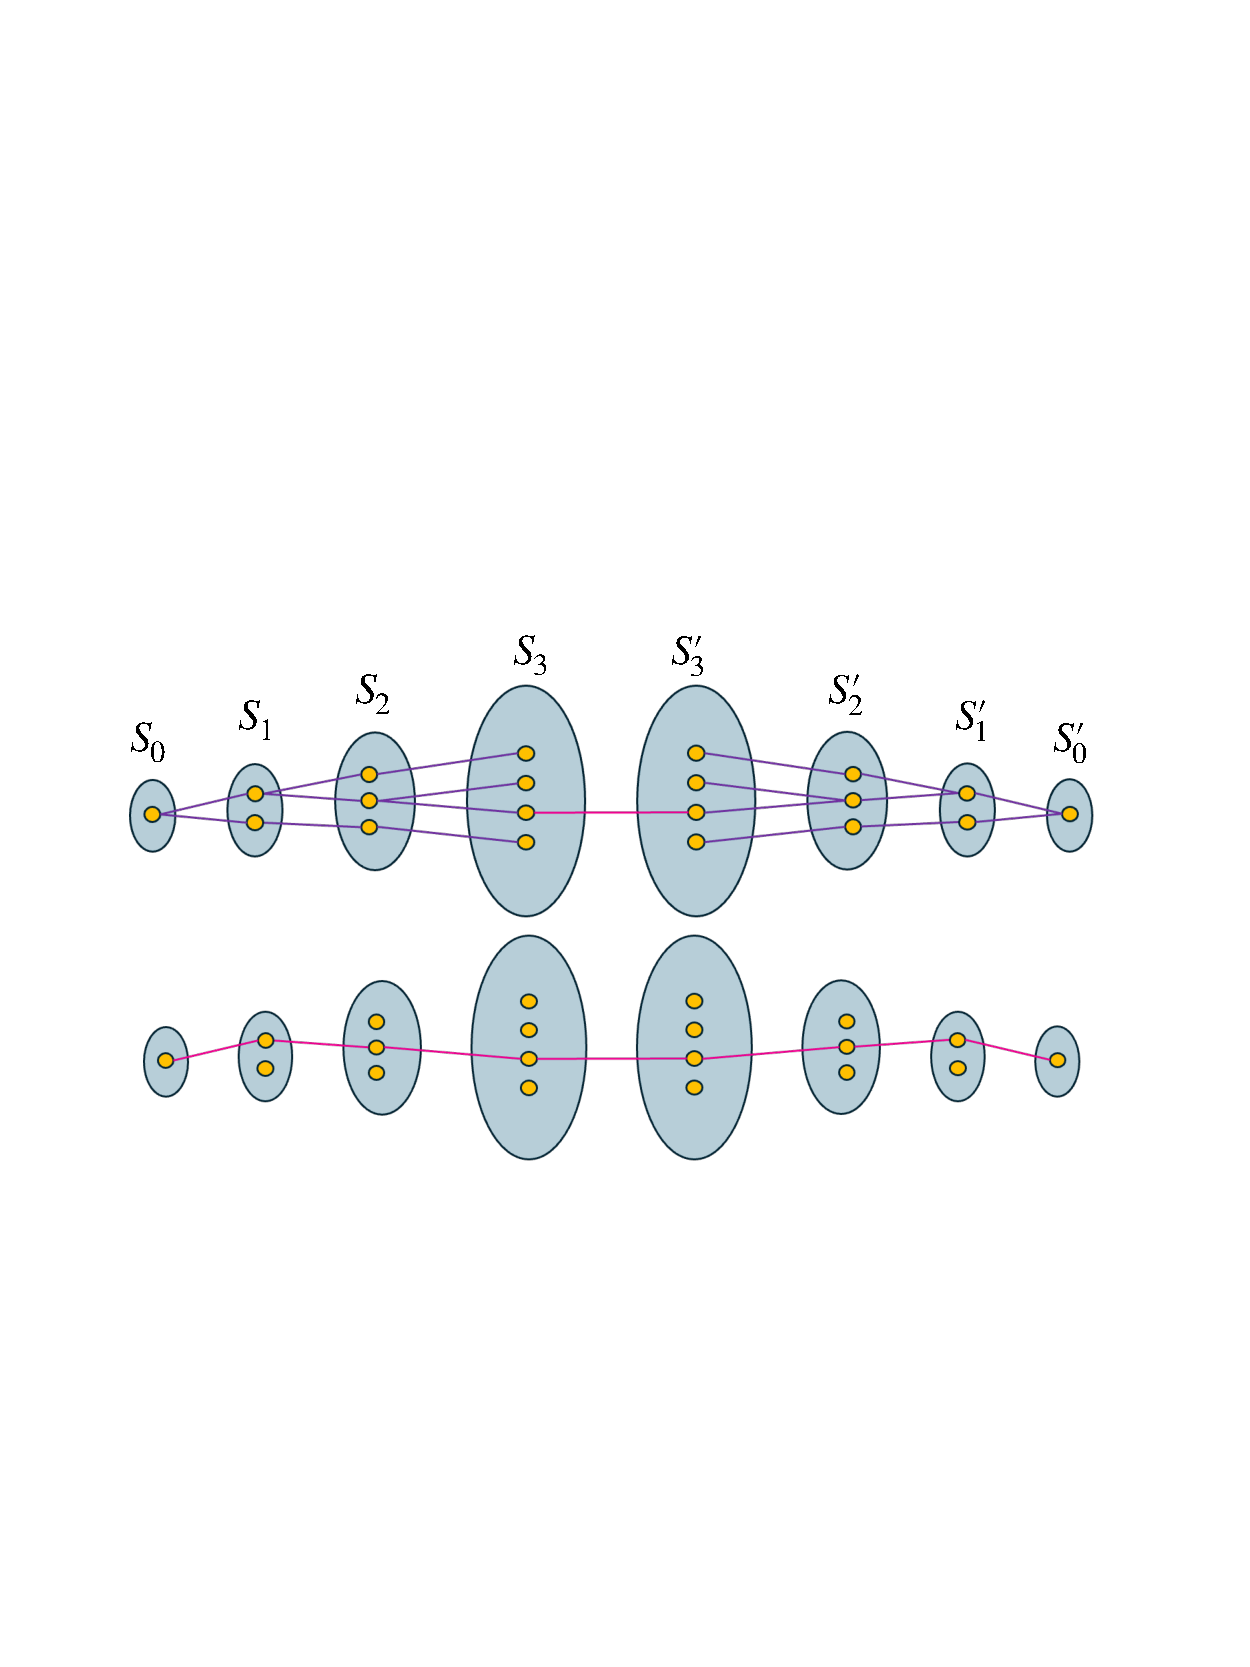
\includegraphics[width=0.9\textwidth
	]{assets/BaseA.pdf}
	\caption{The figure on top describes the forward phase of finding sets $\{M_i\}_{i\in [k]}$ and $\{M_i'\}_{i\in [k]}$. The figure on top describes the process of backtracking from the edge $e$ that is promised to exist between $S_k$ and $S_k'$.}
	\label{fig:baseB}
\end{figure}



\paragraph{Induction Step}
	
Assume that we have found paths for $e_1 = (u_1, v_1), \dots, e_j=(u_j, v_j)$ for $j < m$.
Let $P_1, \dots, P_j$ denote these paths (depicted with \textcolor{carminepink}{pink} edges in Figure \ref{fig:induction}) .
Let $\GlobalEdgeSet$ denote the set of all edges in these paths.
Let $e_{j+1} = (u_{j+1},v_{j+1}) \in \Edges{H}$.
Set $S_0 = \{u_1, \dots, u_j\}$ and $S_0' = \{v_1, \dots, v_j\}$
Note that $\GlobalEdgeSet \leq tk \leq \epsilonA n$.
The process for finding a path between $u_{j+1}$ and $v_{j+1}$ reduces the base case, where now for any $1 \leq i \leq k$, for each node in $S_i$ and $S_i'$ we find a safe neighbour that does not have an incident  edge from $E' \cup (\cup_{i=1}^k (M_i \cup M'_i))$. As $|M| < \epsilonA\na$ as well, we are guaranteed safe neighbours exist for each node (depicted with \textcolor{purple}{purple} edges in Figure \ref{fig:induction})).
This concludes the proof.

\begin{figure}
	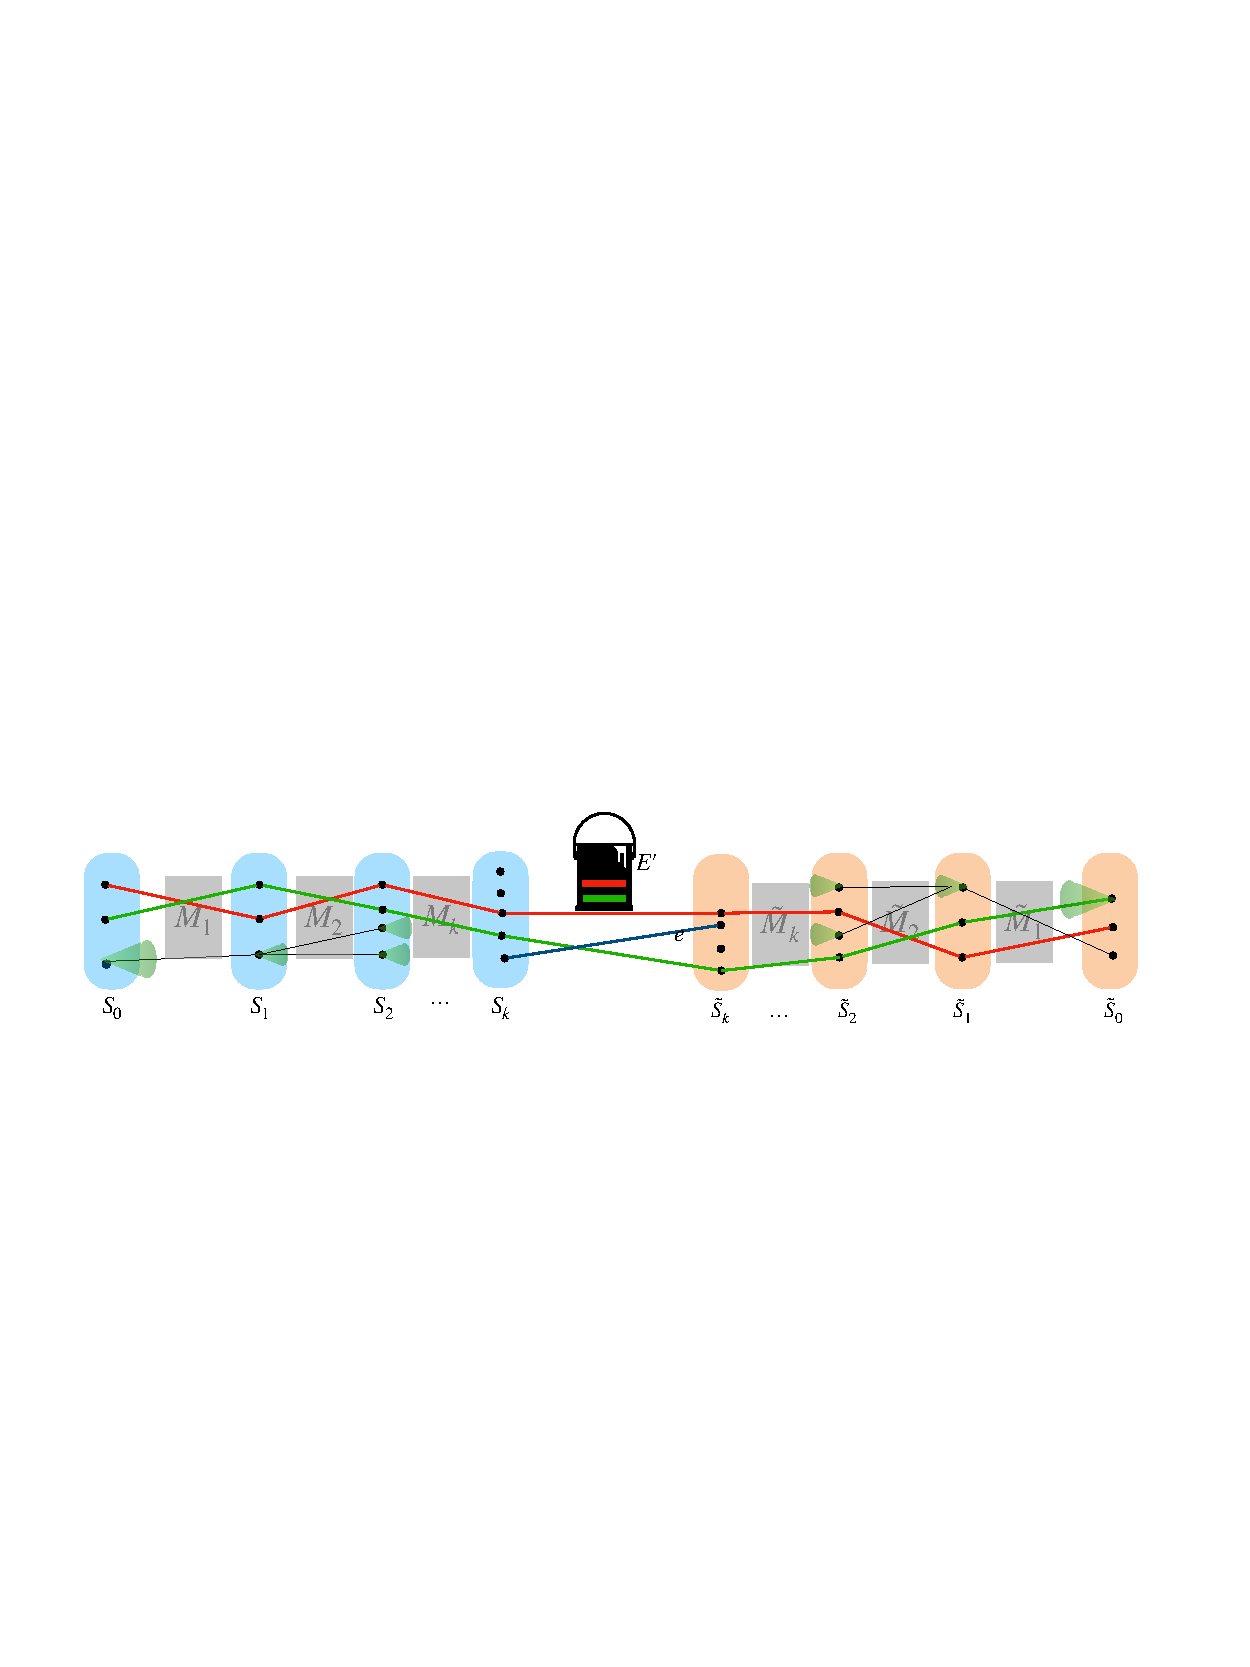
\includegraphics[width=0.9\textwidth
	]{assets/InductionStep.pdf}
	\caption{The figure above describes the induction step. The nodes in green are already in the embedding and represent paths $P_1, \dots, P_j$ for edges $(u_1, v_1) \dots, (u_j, v_j)$.
	The nodes in yellow represent candidates for the path for edge $u_{j+1}, v_{j+1}$. 
	The candidate nodes are constructed identical to the procedure described in the base step of the induction step, where we use the non-blocking property of $\BipartiteG$ to extend with safe neighbours. 
	}
	\label{fig:induction}
\end{figure}

	
\end{proof}

\subsection{Step 3: Finding A Perfect Matching In The Remainder Of The Graph}

\begin{definition}[Edge Connectivity]\label{def:edge-connectivity}
The edge connectivity of a graph $G$, denoted with $\EdgeConnectivity{G}$ is the minimum number of edges we must delete from the graph to make it disconnected.	
\end{definition}

%Lemma \ref{lemma:expanders-minimal-matching} is from \citep[Theorem 4.3]{krivelevich2006pseudo}, that says the pseudorandom graphs on an even number of vertices have perfect matchings.


\ari{Add subgraph notation}
\begin{lemma}[Tutte Criterion]\label{lemma:tutte-criterion}
Let $\OddComponents{G}$ denote the number of odd components in a graph $G=(V,E)$. 
$G$ admits a perfect matching \emph{if and only if} for every $S \subseteq V$, $\OddComponents{G[V \setminus S]} \leq |S|$.
\end{lemma}


\begin{theorem}{Perfect Matching On The Remainder Theorem}{perfect-matching}
Given $\EnDeeLambda$ graph $\Graph=(V,E)$, let $\Embedding{\Subdivision{H}{\sigma}}$ be the topological embedding of the hard instance $H$ from the \nameref{theorem:top-embedding}.
There exits a small constant $\PartitionEps \in (0,1)$, such that 
if $\ExpansionFactor{G} \leq d - \PartitionEps d - 2$, then the sub-graph $\Graph[V \setminus \Embedding{\Subdivision{H}{\sigma}}]$ has a perfect matching.	
	
\end{theorem}


\begin{proof}
Let $\PartitionEps = 2\Eps$, where $\Eps$ is as defined above.
Define $\tilde{d} = d - \Eps d =d - \frac{d\PartitionEps}{2}$ and let $\tilde{G}=(\tilde{V}, \tilde{E})$ be short hand for $\Graph[V \setminus \Embedding{\Subdivision{H}{\sigma}}]$.
Assume that the edge connectivity of $\tilde{G}$, denoted by $\EdgeConnectivity{\tilde{G}}$, is $\tilde{d}$. 
%Then we show using the Tutte criterion that $\tilde{G}$ admits a perfect matching.
Pick arbitrary $S \subseteq \Vertices{\tilde{G}}$.
By the guarantees of the  \nameref{theorem:partition}, 
the minimal degree of $\tilde{G}$ is $\tilde{d}$. 
Therefore, the number of edges in the cut between $S$ and $\Complement{S}$ is at most $\tilde{d}|S|$.
If $\EdgeConnectivity{\tilde{G}} = \tilde{d}$, then by a simple counting argument, it must be that $\OddComponents{\tilde{G}[\tilde{V} \setminus S]} \leq |S|$ (as we need to delete  at least $\tilde{d}$ edges in the cut to disconnect the graph).
Thus, by Lemma \ref{lemma:tutte-criterion}, $\tilde{G}$ admits a perfect matching.

To complete the proof we need to show that $\EdgeConnectivity{\tilde{G}} = \tilde{d}$.
Let $\tilde{n} \Def |\tilde{V}|$.
Pick arbitrary $U \subset \tilde{V} \subset V$ such that $|U| \Def u \leq \tilde{n}/2 \leq n/2$.
As $G$ is an $\EnDeeLambda$ graph, we have

\begin{align}
\CutEdges{U}{\Complement{U}}{E} &\geq 	\frac{d}{n}u(n-u) - \lambda\sqrt{u(n-u)(1 - u/n)(1- (n-u)/n)} \label{eq:step1}\\
&= \frac{(n-u)}{u}u(d - \ExpansionFactor{G}) \label{eq:step2}\\
&\geq \frac{u}{2}(d - \ExpansionFactor{G})
\end{align}

\eqref{eq:step1} comes from the tighter version of the expander mixing lemma (Lemma \ref{lemma:expanders-mixing-lemma}), and 
\eqref{eq:step2} comes from the fact $u \leq n/2$.
To construct $\tilde{G}$, we delete at most $\Eps$ fraction of edges for each vertex $v \in V$, such that the degree of every vertex $v \in \tilde{V}$ is at least $\tilde{d}$.
Therefore, the number of edges across $U$ and $\Complement{U}$ based on $E$ we might have to delete to construct $\tilde{G}$ is at most $u(\PartitionEps d)/2$.

\begin{align}
	\CutEdges{U}{\Complement{U}}{\tilde{E}} &\geq 	\CutEdges{U}{\Complement{U}}{\tilde{E}} - \frac{\PartitionEps d}{2} u \\
&\geq \frac{u}{2}(d - \ExpansionFactor{G}) - \frac{\PartitionEps d}{2} u \\
&= \frac{u}{2}\left(d - \ExpansionFactor{G} - \PartitionEps d\right) \label{eq:lambda-assumption} \\
&\geq \tilde{d}
\end{align}


\eqref{eq:lambda-assumption} comes from the assumption that $\ExpansionFactor{G} \leq d - \PartitionEps d - 2$, which is easily satisfied by the conditions on $\ExpansionFactor{G}$ in the above lemmas.
%be an arbitrary subset of size at most $\tilde{n}/2$.\ari{Make sure to define $\tilde{n}$}.

%Let $\Embedding{\Subdivision{H}{\sigma}}$ denote the subgraph of $G$ which represents the topological embedding of $H$ from Lemma \ref{lemma:top-embedding}.
%Define . 
%That is $\tilde{\Graph}$ is a subgraph of $\Graph$ using all vertices in $B$ and the vertices in $A$ that were not used to embed $\Subdivision{H}{\sigma}$.
%As $\ExpansionFactor{\Graph} \leq \lambda$, and $\tilde{\Graph}$ is a subgraph, we have $\ExpansionFactor{\tilde{\Graph}} \leq \lambda$.
%%\ari{This is super easy to show using basic linear algebra, I can explicitly prove this if you think it's needed.}
%By lemma \ref{lemma:partition}, we know that the minimal degree $\MinimalDegree{\tilde{\Graph}} \geq \tilde{d}$.
%Let $\dbtilde{\Graph}$ denote a subgraph of $\tilde{G}$, where for each $v \in \Vertices{\tilde{\Graph}}$ we retain exactly $\tilde{d}$ of its neighbours.
%It is easy to see that $\dbtilde{\Graph}$ is a $(\tilde{n}, \tilde{d}, \lambda)$ pseudorandom graph, where $\tilde{n} = |\Vertices{\tilde{\Graph}}|$ and $n$ is even (since $|\Vertices{\Graph}|$ is odd and $|\Vertices{\Embedding{\Subdivision{H}{\sigma}}}|$ is also odd). 
%As $\lambda \leq \tilde{d} - 2$, we invoke Lemma \ref{lemma:expanders-minimal-matching} to get that $\dbtilde{G}$ has a perfect matching.
%As $\dbtilde{G}$ is a sub-graph of $\tilde{G}$ with the same vertex set, $\tilde{G}$ also has a perfect matching.
%\ari{Set $\lambda$ here from the embedding lemma and you're done}.
\end{proof}

\section{Related Work}

\clearpage
\bibliographystyle{abbrvnat}
\bibliography{main_paper}
\end{document}
